% ReSPect — ICLR 2027 conference submission (anonymous).
% Built on the official ICLR 2027 shell (iclr2027_conference.tex).
\documentclass{article} % For LaTeX2e
\usepackage{iclr2027_conference,times}

% Optional math commands from https://github.com/goodfeli/dlbook_notation.
\input{math_commands.tex}

\usepackage{hyperref}
\usepackage{url}
\usepackage{graphicx,amsmath,amssymb,amsthm,booktabs}
\graphicspath{{figs/}}
\usepackage{xcolor}
\raggedbottom
\setlength{\textfloatsep}{7pt plus 2pt minus 2pt}
\setlength{\floatsep}{5pt plus 2pt minus 2pt}
\newtheorem{theorem}{Theorem}
\newtheorem{lemma}{Lemma}
\newtheorem{remark}{Remark}

\newcommand{\ie}{\textit{i.e.}}
\newcommand{\eg}{\textit{e.g.}}


\title{ReSPect: Residual Spectral Prediction\\for Training-Free Acceleration of Diffusion Transformers}

% Authors hidden for blind review: keep \iclrfinalcopy commented out.
% Author block intentionally omitted in the submission version.

%\iclrfinalcopy % Uncomment for camera-ready version, but NOT for submission.
\begin{document}

\maketitle

\begin{abstract}
Diffusion transformers underlie current image and video generation models, but incur substantial sampling costs due to iterative denoising.
Training-free caching accelerates sampling through two coupled decisions: which steps to evaluate, and what to substitute for the skipped features. Many existing schedules gate on raw distances between adjacent features, a drift signal with poor signal-to-noise ratio, where stochastic variation masks meaningful drift, while ignoring how the noise level itself evolves along the sampling trajectory. Many existing reconstructors, in turn, rely on local approximation, copying the most recently computed features or extrapolating from a short local history. This approach causes approximation errors to increase with the skip length and sample quality to degrade at high speedups. We propose Residual Spectral Prediction for Efficient Caching of Transformers \textbf{(ReSPect)}, a training-free cache that jointly addresses these limitations through spectrally aligned reuse decisions and residual trajectory prediction. Scheduling decisions are based on a spectrally aligned representation obtained from a timestep-dependent filter derived from the linear minimum mean square error (linear-MMSE) denoising formulation, which preserves content-relevant components while suppressing noise. Skipped residuals, rather than hidden states, are forecast by a weighted sum of ridge-regularized Chebyshev regression over the accumulated residual history, which captures the global trajectory, and a first-order discrete Taylor correction, which captures local dynamics. Analysis shows the forecast error admits a skip-length-independent bound, whereas the corresponding bounds for copy-reuse and Taylor extrapolation grow with skip length. Across extensive experiments on FLUX.1-dev, Wan2.1-1.3B, and HunyuanVideo, ReSPect achieves speedups of $3.30\times$, $2.63\times$, and $2.77\times$ over full denoiser evaluation while achieving lower output error than existing caching baselines at matched or lower compute.

\end{abstract}

% \textbf{Keywords:} Generative models; diffusion transformers;
% training-free inference acceleration; feature caching.



\begin{figure}[h]
\vspace{-3mm}
\centering

\includegraphics[width=\linewidth]{figs/teaser_collage.pdf}
\caption{Qualitative visual results of ReSPect on FLUX.1-dev, maintaining high image fidelity at a $2.43\times$ acceleration.}
\label{fig:teaser}
\end{figure}


\section{Introduction}
\label{sec:intro}

Diffusion transformers~\citep{dit} form the backbone of many text-to-image and
text-to-video models~\citep{flux,wan,hunyuanvideo}, and sampling them
requires tens of sequential evaluations of a large transformer network
per output~\citep{ddpm,ddim}. Feature caching reduces this cost without
retraining by exploiting redundancy along the sampling trajectory.

A cache consists of two decisions at every step: a \emph{schedule}
determines whether the network is evaluated, and a \emph{reconstructor}
determines what is written to the features when it is not. The two are
coupled through the skip length. The schedule decides \emph{where} the
model can skip without changing the generated content; the reconstructor
decides \emph{how far} a skip can extend before the substituted features
depart from the uncached trajectory. Improving either in isolation
leaves the other as the bottleneck: a content-aware gate cannot preserve
quality on long skips if the skipped features remain a stale copy, and a
long-horizon predictor cannot be applied aggressively if the gate
responds to noise rather than to content.

Many existing schedules gate on the raw distance between consecutive
features~\citep{teacache,dicache}, which mixes meaningful evolution with
high-frequency noise; others use motion cues~\citep{adacache}, frequency
bands~\citep{freqca}, finer granularity~\citep{deltadit,toca}, or
spectrally filtered distances~\citep{seacache}. The relevant insight is
that a timestep-dependent spectral filter isolates content-sensitive
drift, so the gate responds to changes in the generated content rather
than to stochastic variation (Sec.~\ref{sec:gate}). Many existing
reconstructors rely on local temporal information, such as feature reuse~\citep{fora,pab} or finite-difference extrapolation~\citep{taylorseer}, while global trajectory fitting methods still predict the full hidden
state~\citep{spectrum}. Rather than forecasting the hidden state itself,
we forecast only the transformer residual, because the block input at
skipped steps is known exactly. This removes the predictable component
from the regression target and yields a smaller, centered trajectory
(Sec.~\ref{sec:residual}).

We present \textbf{ReSPect} (Residual Spectral Prediction for Efficient
Caching of Transformers), a training-free cache that models cache
decisions and skipped-step dynamics from spectrally filtered drift and
residual trajectory history (Fig.~\ref{fig:framework}). The resulting
predictor models the residual trajectory from the full observed history,
combining a global Chebyshev estimate with a local Taylor correction.
Both the blend and the warm-up are analytically determined
(Sec.~\ref{sec:blend}).

Our contributions are as follows.
\begin{itemize}
\item We formulate cache reconstruction as residual-trajectory
  prediction and rank reconstructors by their error bounds linear in
  the skip length for copy-reuse, order $P{+}1$ for ideal order-$P$
  Taylor, skip-length independent for a ridge-regularized Chebyshev
  fit~\citep{spectrum} and refine the Taylor case for the non-uniform
  evaluation nodes a dynamic gate produces (Sec.~\ref{sec:hierarchy}).
\item We show that state and residual forecasts share the same error
  identity on a skipped step, but that residuals are substantially
  smaller in norm, which tightens the constant $B$ in the ridge
  analysis and motivates residual-space prediction
  (Sec.~\ref{sec:residual}).
\item We derive the blend weight and the warm-up length in closed form
  from bias--variance and degrees-of-freedom arguments, eliminating two
  hyperparameter searches (Sec.~\ref{sec:blend}).
\end{itemize}
Coupling the residual forecaster with a spectrally aligned,
content-aware schedule, we demonstrate improved quality-compute
trade-offs against published caching baselines on FLUX.1-dev,
Wan2.1-1.3B, and HunyuanVideo, with every comparison made at matched or
lower compute (Sec.~\ref{sec:exp}).

% FIGURE 2: method overview
\begin{figure}[t]
  \centering
  \includegraphics[width=\linewidth]{pipeline.png}
  \caption{\textbf{Overview of ReSPect.}
(a) Spectrally aligned gate for adaptive compute decisions.
(b) Residual forecaster combining global Chebyshev prediction with a
local first-order Taylor correction.}
  \label{fig:framework}
\end{figure}

\section{Related Work}
\label{sec:related}

\paragraph{Accelerating diffusion sampling.}
Diffusion models~\citep{ddpm,ddim} and latent diffusion
models~\citep{ldm}, together with transformer-based
denoisers~\citep{dit}, form the foundation of many modern
text-to-image~\citep{flux} and text-to-video
models~\citep{wan,hunyuanvideo}. A broad range of approaches has been
developed to reduce their inference cost, including
distillation~\citep{consistency,dmd},
quantization~\citep{li2023q,zhao2024vidit},
efficient attention mechanisms, and accelerated numerical
solvers~\citep{ddim,dpm}. These approaches typically require additional
training, model modification, or changes to the sampling procedure.
Feature caching is complementary to these approaches: it reduces
redundant network evaluations during sampling without retraining the
underlying generative model.

\paragraph{Skip schedules.}
Early caches evaluate the network at fixed intervals~\citep{fora,pab}.
Dynamic schedules instead gate on a redundancy signal: the distance
between consecutive features~\citep{teacache,dicache},
motion~\citep{adacache}, or frequency-band energy~\citep{freqca}, while
block-level~\citep{deltadit} and token-level~\citep{toca} caches vary
the granularity of reuse. SeaCache~\citep{seacache} improves the
scheduling signal by measuring redundancy after a timestep-aware
spectral filter, but retains feature reuse for skipped steps.

\paragraph{Skip reconstructors.}
Copy-reuse is zero-order prediction; TaylorSeer~\citep{taylorseer}
extrapolates hidden states from finite differences of recent
evaluations (local forecasting); Spectrum~\citep{spectrum} regresses
hidden-state trajectories on Chebyshev bases (long-range
forecasting). SeaCache and Spectrum are the closest prior methods
from complementary directions: spectrally aligned scheduling (when
to evaluate) and Chebyshev forecasting (what to substitute).
ReSPect differs on both axes: it forecasts the transformer residual
rather than the full hidden state, blends the global Chebyshev fit
with a local Taylor correction, and couples the predictor with a
content-aware spectral schedule (Sec.~\ref{sec:method}).


\section{Method}
\label{sec:method}

\subsection{Problem setup}
\label{sec:setup}
We consider a latent generative model whose sampling trajectory
$\{x_t\}_{t=0}^{T}$ is produced by a discrete solver. Here
$t \in \{0,\ldots,T\}$ denotes the sampling/solver index, and the
sequence is traversed in the model's reverse or flow direction, from the
initial noisy state toward the clean output. Each step evaluates a
transformer network, so sampling costs $T$ forward passes.

At each solver step $t$, the current latent $x_t$ is mapped to the
input $I_t = \phi(x_t, t)$ of a transformer block, whose output
$h_{\mathrm{out}}(t)$ is produced from input $h_{\mathrm{in}}(t)$. The
block residual
\begin{equation}
  r(t) = h_{\mathrm{out}}(t) - h_{\mathrm{in}}(t)
\end{equation}
induces a second trajectory $\{r(t)\}$ alongside $\{x_t\}$. Adjacent
solver states often exhibit substantial temporal redundancy, and this
redundancy propagates to intermediate transformer features.

To derive the spectral gate we model the latent at step $t$ as the
linear mixture
\begin{equation}
  x_t = a_t x_0 + b_t \varepsilon, \qquad
  \varepsilon \sim \mathcal{N}(0, I),
\end{equation}
where $x_0$ is the clean latent, $(a_t, b_t)$ are the signal and noise
coefficients at that solver step, and $\varepsilon$ is white and
independent of $x_0$. This is a signal/noise model for the gate, not a
claim that every evaluated architecture follows this exact probabilistic
forward process; flow schedules enter by reading $(a_t, b_t)$ from the
solver (Appendix~\ref{app:wiener}).

A cache consists of two decisions at every step. A \emph{schedule}
determines whether the network is evaluated at step $t$, and a
\emph{reconstructor} determines what is written to the features when it
is not. On an evaluated step the identity
$h_{\mathrm{out}}(t) = h_{\mathrm{in}}(t) + r(t)$ holds by definition.
On a skipped step the input $h_{\mathrm{in}}(t)$ is known, and the
reconstructor supplies $\hat{r}(t)$, yielding
\begin{equation}
  \hat{h}_{\mathrm{out}}(t) = h_{\mathrm{in}}(t) + \hat{r}(t).
\end{equation}
The reconstruction error therefore coincides with the residual error,
\begin{equation}
  \hat{h}_{\mathrm{out}}(t) - h_{\mathrm{out}}(t)
  = \hat{r}(t) - r(t).
\end{equation}
ReSPect specifies both decisions: a spectrally aligned gate
(Sec.~\ref{sec:gate}) and a residual forecaster
(Secs.~\ref{sec:hierarchy}--\ref{sec:blend});
Fig.~\ref{fig:framework} gives an overview.

\subsection{Spectrally aligned gate: when to compute}
\label{sec:gate}
A dynamic gate skips the network while the filtered representation
changes slowly and triggers a full evaluation once the accumulated
drift exceeds a threshold $\delta$. Because the gate is evaluated at
every solver step, it must incur negligible overhead. We therefore
compute it from the first-block input $I_t = \phi(x_t, t)$, which is
available before executing the transformer blocks, and measure the
relative $\ell_1$ distance between consecutive steps, as in prior
distance-gated caches~\citep{teacache}:
\begin{equation}
  \Delta_t = \mathrm{L1}_{\mathrm{rel}}(I_t, I_{t+1})
  = \frac{\|I_t - I_{t+1}\|_1}{\|I_{t+1}\|_1 + \xi}.
\end{equation}
This raw distance is a noise-contaminated drift: under the mixture
above, the noise contribution can dominate the raw distance at early
steps, so $\Delta_t$ responds to stochastic variation on which no cache
decision should depend. We therefore pass from the raw representation
to a spectrally filtered drift, measuring distance on the component of
$I_t$ that is aligned with the clean signal. The linear-MMSE estimator
of $x_0$ from $x_t$,
\begin{equation}
 h_t^\star = \arg\min_h\, \|h \ast x_t - x_0\|_2^2,
  \label{eq:mmse}
\end{equation}
is convolutional, so its solution is diagonal in the Fourier domain and
yields the Wiener frequency response
\begin{equation}
  G_t(f) = \frac{a_t S_x(f)}{a_t^2 S_x(f) + b_t^2},
  \label{eq:wiener}
\end{equation}
where $S_x$ is the power spectrum of the clean latent. Under a
power-law spectral prior $S_x(f) \propto 1/|f|^p$, $G_t$ passes only
low frequencies at early steps (small $a_t$) and admits progressively
higher frequencies as sampling proceeds toward the clean output,
reproducing the observed spectral evolution along the sampling
trajectory, in which coarse structure is formed first and fine detail
later (Fig.~\ref{fig:app-filters}; Appendix~\ref{app:wiener}). Applying
$G_t$ to $I_t$ in the Fourier domain yields
$\mathcal{P}(G_t, I_t)
= \mathcal{F}^{-1}\!\big[G_t \odot \mathcal{F}(I_t)\big]$,
a representation whose drift reflects content change with the noise
component suppressed.

The raw responses $G_t$ differ in overall gain across $t$, which would
allow high-gain steps to dominate the accumulator. We therefore
normalize each response to unit mean gain over radial frequency bins,
\begin{equation}
  G_t^{\mathrm{norm}}(f) = \nu_t G_t(f), \quad
  \nu_t^{-1} = \frac{1}{L}\sum_{\ell} G_t(f_\ell),
  \label{eq:norm}
\end{equation}
so that the accumulator measures changes in spectral shape rather than
changes in overall filter gain. Because the optimal spectral response
is timestep-dependent, each adjacent pair is compared using its
corresponding normalized response $G_t^{\mathrm{norm}}$ and
$G_{t+1}^{\mathrm{norm}}$:
\begin{equation}
  \tilde{\Delta}_t = \mathrm{L1}_{\mathrm{rel}}\big(
  \mathcal{P}(G_t^{\mathrm{norm}}, I_t),
  \mathcal{P}(G_{t+1}^{\mathrm{norm}}, I_{t+1})\big)
  \label{eq:gate}
\end{equation}
The gate accumulates $\tilde{\Delta}_t$ and evaluates the transformer
network when the sum exceeds $\delta$, resetting the accumulator; the
first and last steps are always evaluated. Crucially, the reference is
refreshed at every step, including skipped steps, so each
$\tilde{\Delta}_t$ measures only the incremental drift between
consecutive solver states (Sec.~\ref{sec:ablation} quantifies the
difference). The gate decides \emph{which} steps are evaluated; the
remainder of this section specifies \emph{what} is written on the
others.

\subsection{Predictors on the sampling trajectory}
\label{sec:hierarchy}

The reconstruction problem is therefore reduced to forecasting the
residual trajectory at unevaluated steps. We state the analysis for one
residual channel; the predictor is applied independently across
channels. Consider a skip from the last evaluated step $t_k$ to the
current step $t_j$. Every reconstructor is a predictor
$\hat{r}(t_j)$ built from the residuals recorded at evaluated steps;
the candidates differ in the smoothness they assume of $r$.

\paragraph{Order zero (copy-reuse).}
$\hat{r} = r(t_k)$. If $r$ is $L$-Lipschitz, Lipschitz continuity gives
\begin{equation}
  |r(t_j) - r(t_k)| \le L\,|t_j - t_k|,
  \label{eq:reuse}
\end{equation}
which is tight in general and yields a linear error bound in the skip
length (App.~\ref{app:reuse}). No smoothness assumption beyond Lipschitz
continuity can improve the bound, since copy-reuse exploits no
higher-order structure.

\paragraph{Order $P$ (Taylor extrapolation).}
The ideal degree-$P$ Taylor expansion of $r$ about $t_k$ has a
Lagrange remainder of order $|t_j-t_k|^{P+1}$~\citep[Thm.~3.1]{spectrum};
see App.~\ref{app:taylor}. A higher order thus sharpens the bound for
short skips --- but only as an oracle reference, since the exact
derivatives are unavailable in a training-free cache. The implemented
predictor interpolates recorded residuals instead, and recovers the
$(P{+}1)$-order rate only under comparable node spacing, which the
dynamic gate does not guarantee (App.~\ref{app:taylor}). Taylor
extrapolation is therefore
accurate when the skip is short but its remainder grows with the
extrapolation distance; it also discards older trajectory information.
These bounds motivate a global predictor that can exploit the full
observed trajectory rather than only local finite differences;
Sec.~\ref{sec:cheb} develops such a predictor using a
ridge-regularized Chebyshev basis.

\subsection{Residual forecasting with Chebyshev bases}
\label{sec:cheb}
To predict $r(t_j)$, we fit the accumulated residual trajectory. Map
the solver-step index affinely from the fixed solver-step range to
$\tau \in [-1,1]$, and expand each residual channel (of feature
dimension $F$) in the Chebyshev basis $T_0,\dots,T_M$ of degree $M$.
Stack the $K$ recorded residuals row-wise into the observation matrix
$\mathbf{H} \in \mathbb{R}^{K \times F}$, let
$\mathbf{\Phi} \in \mathbb{R}^{K \times (M+1)}$ evaluate the basis at
the recorded steps, and regress the coefficient matrix
$\mathbf{C} \in \mathbb{R}^{(M+1) \times F}$ with ridge penalty
$\lambda$:
\begin{equation}
  \mathbf{C}^\star = \arg\min_{\mathbf{C}}
  \|\mathbf{\Phi}\mathbf{C} - \mathbf{H}\|_F^2
  + \lambda\|\mathbf{C}\|_F^2
  = (\mathbf{\Phi}^\top\mathbf{\Phi} + \lambda I)^{-1}
    \mathbf{\Phi}^\top \mathbf{H}.
  \label{eq:ridge}
\end{equation}
Each row of $\mathbf{\Phi}$ evaluates the basis at one recorded step,
and the corresponding row of $\mathbf{H}$ holds the recorded residual.
The fit is re-solved whenever a new residual is computed; the window
retains the last $K$ observations, which exceeds the number of solver
steps in all reported runs. The forecast at a skipped step
evaluates the fitted expansion at its coordinate,
$\hat{r}(t_j) = \sum_{m=0}^{M} \hat{C}_m\,T_m(\tau_j)$. Let
$p_M^\star$ denote the exact degree-$M$ Chebyshev truncation of $r$.
Under the standard analyticity assumption that $r$ extends analytically
to a Bernstein ellipse of parameter $\rho>1$ on which $|r| \le B$,
classical Chebyshev approximation gives~\citep[Thm.~3.2]{spectrum}
\begin{equation}
  \|r - p_M^\star\|_\infty \le \frac{2B}{\rho-1}\,\rho^{-M},
  \label{eq:cheb}
\end{equation}
uniformly in the evaluation point (App.~\ref{app:cheb}): this
truncation term decays with the degree $M$ and is independent of the
skip length. Because the coefficients are estimated from finitely many
observations, we also control the deviation of the estimator from that
ideal truncation.

\begin{lemma}[{Ridge stability, restated from \citealt[Thm.~3.3]{spectrum}}]
\label{lem:ridge}
Let $\hat{r}$ be the Chebyshev component from~\eqref{eq:ridge} and
$p_M^\star$ the exact degree-$M$ truncation. With
$\sigma_{\min} = \sigma_{\min}(\mathbf{\Phi})$, equal to zero whenever
$K < M{+}1$, at any forecast coordinate $\tau_j$,
\begin{equation}
  |\hat{r}(\tau_j) - p_M^\star(\tau_j)| \le
  \varepsilon_M \frac{(M{+}1)K}{\sigma_{\min}^2 + \lambda}
  + \frac{\lambda\sqrt{M{+}1}}{\sigma_{\min}^2 + \lambda}
    \cdot \frac{2B}{\sqrt{1-\rho^{-2}}},
\end{equation}
for $\varepsilon_M$ the right-hand side of~\eqref{eq:cheb}; with that
equation and the triangle inequality this bounds the total error
$|r(\tau_j) - \hat{r}(\tau_j)|$ (App.~\ref{app:ridge}).
\end{lemma}
Each observation adds a positive semi-definite rank-one term to
$\mathbf{\Phi}^\top\mathbf{\Phi}$, so $\sigma_{\min}$ is non-decreasing
in $K$ and the factor $K/(\sigma_{\min}^2 + \lambda)$ stays bounded
rather than growing; before $K$ reaches $M{+}1$ the design is
rank-deficient and $\lambda$ alone controls the bound, at the price of
bias. Sec.~\ref{sec:blend} turns this stability condition into an
explicit warm-up threshold.

\subsection{Residual space}
\label{sec:residual}
On a skipped step, the block input $h_{\mathrm{in}}$ is known exactly
from the current sampling state and the preceding computation; it
therefore does not need to be forecast. For a state forecast
$\hat{h}_{\mathrm{out}}$ and a residual forecast $\hat{r}$,
\begin{equation}
  \hat{h}_{\mathrm{out}} - h_{\mathrm{out}}
  = (\hat{r} + h_{\mathrm{in}}) - (r + h_{\mathrm{in}})
  = \hat{r} - r.
\end{equation}
Thus, once the predictor is fixed, state and residual formulations have
identical reconstruction error; they differ only in their regression
target. The full hidden state carries a large component that is already
determined by $h_{\mathrm{in}}$, so fitting it forces the regression to
reproduce variation the sampler already knows and inflates the target
scale. The residual trajectory is substantially smaller in norm, so
comparable relative fit quality yields smaller absolute error and
tighter constants in the ridge analysis (Lemma~\ref{lem:ridge}), whose
constant $B$ scales with the target norm. This comparison takes the
residual trajectory to satisfy the same analyticity condition with
comparable $\rho$; consistent with this, the $M$-sweep in
 Tab.~\ref{tab:abl-M} saturates at the same small $M$ used
throughout. The skipped-step update is simply $h \leftarrow h + \hat{r}$: the
forecast supplies the missing transformer increment, and no full
network evaluation is needed.
\subsection{Analytic blend and warm-up}
\label{sec:blend}

\paragraph{Blend.}
For the risk model, we assign the Taylor predictor's systematic
error to bias $b_T^2$ and the Chebyshev estimator's finite-history
uncertainty to variance $\sigma_C^2$, and omitting
$w$-independent terms, the risk of the
convex combination $\hat{r}_w = (1-w)\hat{r}_T + w\hat{r}_C$ is
\begin{equation}
  R(w) = (1-w)^2 b_T^2 + w^2 \sigma_C^2,
\end{equation}
minimized at $w^\star = b_T^2/(b_T^2 + \sigma_C^2)$. Early in sampling
the drift is fast ($b_T$ large) and the fit has seen few points
($\sigma_C$ large); later both decrease as the trajectory settles and
observations accumulate. Thus Taylor is relatively more reliable
during the early sparse-history regime, while the global Chebyshev
predictor becomes increasingly reliable as observations accumulate.
Because the bias and variance terms are not observable at inference
time, we cannot evaluate $w^\star$ online and instead use the
symmetric fixed weight $w{=}0.5$, which introduces no additional
inference-time adaptation or hyperparameter search. The ablations in
App.~\ref{app:abl-reuse} show that this choice remains robust across
models and budgets, staying close to the stronger component on each
model, whereas $w{=}1$ removes the low-bias local term precisely when
the polynomial fit is least determined.

\paragraph{Warm-up.}
With $n < M{+}1$ observations, \eqref{eq:ridge} is rank-deficient
($\sigma_{\min} = 0$) and the penalty dominates the data, so ReSPect
uses the discrete Taylor step alone: exact on the most recent points
by construction, it reduces to copy-reuse at $n = 1$ and extrapolates
linearly from $n = 2$ onward. In practice the regularized fit is
determined one observation early, so blending starts at $n \ge 4$
(with $M{=}4$) rather than $M{+}1$.
\paragraph{Compute and memory.}
Skip decisions accumulate per sample, so prompts in a batch never share
a schedule. Each sample stores one $(M{+}1)\times F$ coefficient matrix
and $K$ recorded residuals, i.e.\ $\mathcal{O}((M{+}1)F + KF)$ memory
and $\mathcal{O}(K(M{+}1)F)$ fitting cost with $M \ll K \ll F$, which
is negligible relative to a transformer block (${\sim}0.09$\,s per image
in our runs).

% \begin{figure}[t]
%   \centering
%   \fbox{\parbox{0.95\linewidth}{\small
%   Initialize accumulator $a{=}0$ and forecaster
%   $\mathcal{F}{=}\emptyset$; force full evaluation at $t{=}0,T{-}1$.
%   \textbf{For} $t=0\dots T{-}1$: $a \mathrel{+}= \tilde{\Delta}_t$;
%   full $\gets (a \ge \delta)$ (reset $a$ if full); \textbf{if} full: run
%   blocks, $r_{\mathrm{prev}} \gets h_{\mathrm{out}} - h_{\mathrm{in}}$,
%   $\mathcal{F}.\mathrm{update}(t, r_{\mathrm{prev}})$; \textbf{else}:
%   $h \gets h + \mathcal{F}.\mathrm{predict}(t)$ (fall back to
%   $r_{\mathrm{prev}}$ if no observations exist; Taylor-only while
%   $n<4$).}}
%   \caption{ReSPect sampling (per sample). The filtered
%   distance~\eqref{eq:gate} selects the evaluated steps; the residual
%   forecaster of Secs.~\ref{sec:cheb}--\ref{sec:blend} fills the
%   skipped ones. Samples in a batch are scheduled independently.}
%   \label{fig:algo}
% \end{figure}

\begin{table}[t]
  \centering
  \caption{FLUX.1-dev, DrawBench 200, $1024{\times}1024$, 50 steps. Speedup is Original latency ($5.31$\,s) over row latency.
  ReSPect spends equal or less compute than every baseline in its block.}
  \label{tab:flux}
  \vspace{0.1cm}
  {\small\setlength{\tabcolsep}{4pt}
  \begin{tabular}{lccccc}
    \toprule
    Method & PSNR$\uparrow$ & SSIM$\uparrow$ & LPIPS$\downarrow$ & Lat.\ (s) & Speedup \\
    \midrule
    Original (50 steps) & -- & -- & -- & 5.31 & $1.00\times$ \\
    \midrule
    Vanilla 25 steps & 15.55 & 0.668 & 0.409 & 2.72 & $1.95\times$ \\
    TeaCache ($\delta{=}0.3$) & 20.76 & 0.810 & 0.211 & 2.85 & $1.86\times$ \\
    TaylorSeer ($\mathcal{S}{=}3$) & 22.78 & 0.828 & 0.163 & 2.52 & $2.11\times$ \\
    \textbf{ReSPect ($\delta{=}0.37$)} & \textbf{26.24} & \textbf{0.895} & \textbf{0.093} & \textbf{2.19} & {$2.43\times$} \\
    \midrule
    Vanilla 15 steps & 17.84 & 0.740 & 0.305 & 1.68 & $3.16\times$ \\
    ToCa & 18.40 & 0.700 & 0.324 & 2.25 & $2.36\times$ \\
    TeaCache ($\delta{=}0.6$) & 17.21 & 0.714 & 0.348 & 1.72 & $3.09\times$ \\
    TaylorSeer ($\mathcal{S}{=}5$) & 19.97 & 0.762 & 0.236 & 1.95 & $2.72\times$ \\
    \textbf{ReSPect ($\delta{=}0.6$)} & \textbf{21.63} & \textbf{0.823} & \textbf{0.178} & \textbf{1.61} & \textbf{$3.30\times$} \\
    \bottomrule
  \end{tabular}}
\end{table}


\section{Experiments}
\label{sec:exp}

\subsection{Settings}
\label{sec:settings}
We evaluate FLUX.1-dev~\citep{flux} on 200 DrawBench
prompts~\citep{drawbench} ($1024{\times}1024$, 50 steps) and
HunyuanVideo~\citep{hunyuanvideo} and Wan2.1-1.3B~\citep{wan} on 946
VBench prompts~\citep{vbench} (480p, 65 frames, 50 steps). Metrics are
PSNR, SSIM~\citep{ssim}, and LPIPS~\citep{lpips} against the uncached
same-seed reference. All qualities and latencies are measured on a single NVIDIA B200
(bf16). Each ReSPect operating point uses equal or less compute than
the baseline row it is compared against. Protocol details are in
Appendix~\ref{app:impl}.

\subsection{Text-to-image}
\label{sec:t2i}
On FLUX (Tab.~\ref{tab:flux}), ReSPect attains $26.24$\,dB at
$\delta{=}0.37$, $+3.46$\,dB over TaylorSeer at lower latency (2.19\,s
vs.\ 2.52\,s), and $21.63$\,dB at $\delta{=}0.6$, $+1.66$\,dB while
faster (1.61\,s vs.\ 1.95\,s). Both points dominate the published
quality--compute frontier (Fig.~\ref{fig:curves}).
Fig.~\ref{fig:qual-flux} shows two DrawBench prompts at the aggressive
budget.

\begin{figure}[h]
  \vspace{-2mm}
  \centering
  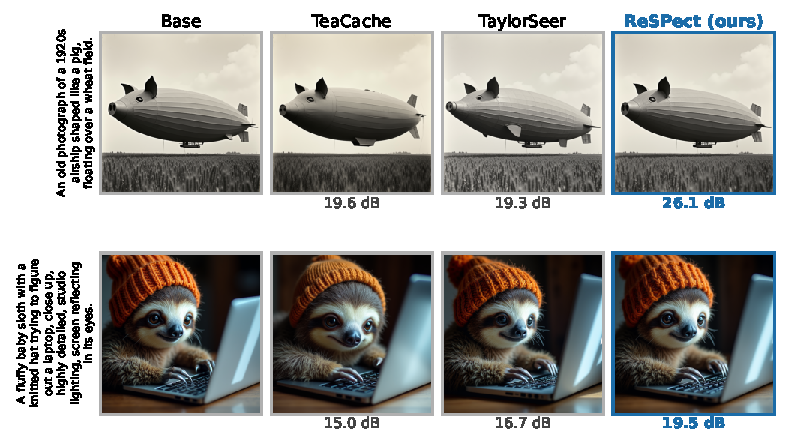
\includegraphics[width=0.78\linewidth]{figs/fig_qual_flux_main.pdf}
  \vspace{-1mm}
  \caption{FLUX.1-dev, $\delta{=}0.6$. PSNR vs.\ the uncached image
  under each panel. TeaCache and TaylorSeer use equal or more compute.}
  \label{fig:qual-flux}
\end{figure}

\begin{figure}[t]
  \centering
  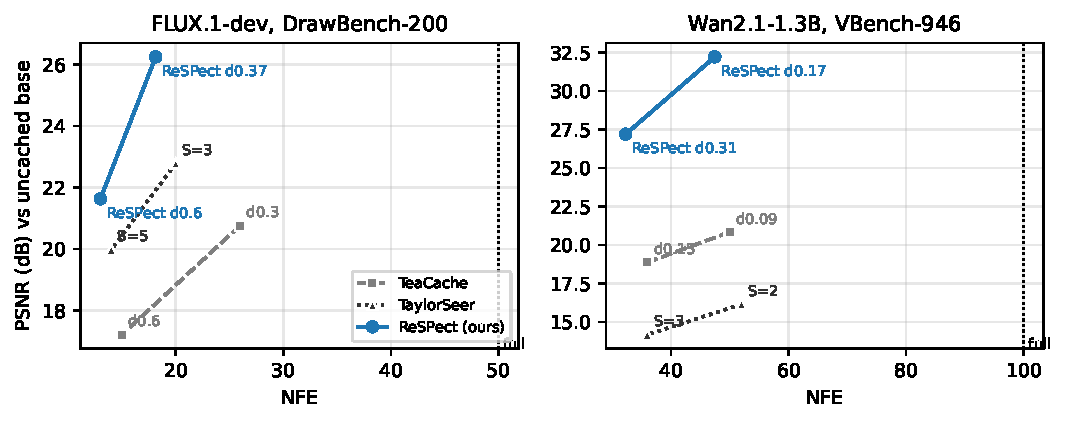
\includegraphics[width=0.85\linewidth]{fig2_quality_compute.pdf}
  \caption{PSNR versus compute. ReSPect is compared with published
TeaCache and TaylorSeer points; dotted line: uncached compute.
The Wan aggressive-budget gain is $+8.32$\,dB.}
  \label{fig:curves}
\end{figure}

\subsection{Text-to-video}
\label{sec:t2v}
Gains are largest on video (Tab.~\ref{tab:video}). On Wan, ReSPect
reaches $32.21$\,dB at $\delta{=}0.17$ ($+11.4$\,dB over TeaCache) and
$27.20$\,dB at $\delta{=}0.31$ ($+8.3$\,dB); LPIPS is less than a third
of any baseline. On HunyuanVideo the margins are $+9.9$\,dB and
$+8.8$\,dB at $\delta{=}0.27$ and $0.48$. Fig.~\ref{fig:video} shows
opening frames; 65-frame strips are in App.~\ref{app:qual}.

\begin{figure}[t]
  \centering
  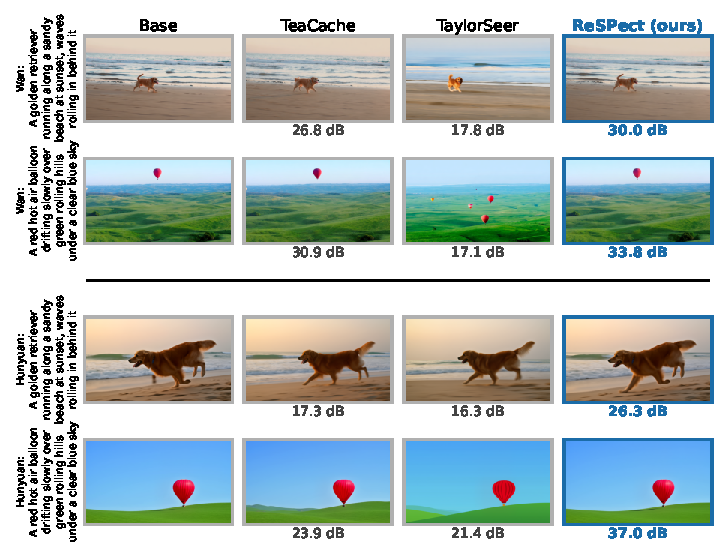
\includegraphics[width=0.9\linewidth]{figs/fig_firstframe.pdf}
  \caption{Opening frames on Wan and HunyuanVideo. ReSPect uses
$\delta{=}0.31/0.48$ with less compute. PSNR is shown below each panel;
full strips are in App.~\ref{app:qual}.}
  \label{fig:video}
\end{figure}

\begin{table}[t]
  \centering
 \caption{Text-to-video results on VBench (480p, 65 frames, 50 steps).
Latencies are measured on one NVIDIA B200 (bf16); speedup is relative
to the Original latency (Hunyuan 77.3\,s, Wan 28.8\,s).}
  \label{tab:video}
  \vspace{0.05cm}
  \begin{minipage}[t]{0.49\linewidth}
    \centering \textit{HunyuanVideo} (Orig.\ 77.3\,s) \\ \vspace{0.05cm}
    {\scriptsize\setlength{\tabcolsep}{2.2pt}
    \resizebox{\linewidth}{!}{%
    \begin{tabular}{lcccc}
      \toprule
      Method & PSNR$\uparrow$ & SSIM$\uparrow$ & LPIPS$\downarrow$ & Lat.\ (s) / Speedup \\
      \midrule
      Original & -- & -- & -- & 77.3 / $1.00\times$ \\
      \midrule
      Vanilla 25 & 19.97 & 0.731 & 0.263 & 38.7 / $2.00\times$ \\
      TeaCache 0.12 & 23.40 & 0.805 & 0.133 & 42.0 / $1.84\times$ \\
      TaylorSeer S2 & 24.14 & 0.820 & 0.152 & 42.0 / $1.84\times$ \\
      \textbf{ReSPect 0.27} & \textbf{34.07} & \textbf{0.946} & \textbf{0.046} & 39.9 / \textbf{$1.94\times$} \\
      \midrule
      Vanilla 15 & 17.49 & 0.662 & 0.371 & 23.2 / $3.33\times$ \\
      TeaCache 0.2 & 20.42 & 0.734 & 0.172 & 30.2 / $2.56\times$ \\
      TaylorSeer S3 & 20.42 & 0.733 & 0.242 & 30.2 / $2.56\times$ \\
      \textbf{ReSPect 0.48} & \textbf{29.20} & \textbf{0.891} & \textbf{0.100} & 27.9 / \textbf{$2.77\times$} \\
      \bottomrule
    \end{tabular}}}
  \end{minipage}\hfill
  \begin{minipage}[t]{0.49\linewidth}
    \centering \textit{Wan2.1-1.3B} (Orig.\ 28.8\,s) \\ \vspace{0.05cm}
    {\scriptsize\setlength{\tabcolsep}{2.2pt}
    \resizebox{\linewidth}{!}{%
    \begin{tabular}{lcccc}
      \toprule
      Method & PSNR$\uparrow$ & SSIM$\uparrow$ & LPIPS$\downarrow$ & Lat.\ (s) / Speedup \\
      \midrule
      Original & -- & -- & -- & 28.8 / $1.00\times$ \\
      \midrule
      TeaCache 0.09 & 20.84 & 0.721 & 0.171 & 14.9 / $1.93\times$ \\
      TaylorSeer S2 & 16.15 & 0.543 & 0.336 & 15.3 / $1.88\times$ \\
      \textbf{ReSPect 0.17} & \textbf{32.21}  & \textbf{0.947}  & \textbf{0.033}  & 14.8 / \textbf{$1.95\times$} \\
      \midrule
      TeaCache 0.15 & 18.88 & 0.645 & 0.245 & 10.4 / $2.77\times$ \\
      TaylorSeer S3 & 14.18 & 0.453 & 0.455 & 11.2 / $2.57\times$ \\
      \textbf{ReSPect 0.31} & \textbf{27.20}  & \textbf{0.888}  & \textbf{0.082}  & 10.9 / \textbf{$2.63\times$} \\
      \bottomrule
    \end{tabular}}}
  \end{minipage}
\end{table}

\subsection{Ablations}
\label{sec:ablation}
On FLUX $\delta{=}0.6$ (first $20$ prompts, fixed across arms with one
shared base run), varying $M$ and $\lambda$ around the defaults yields
a flat optimum (Tabs.~\ref{tab:abl-M}--\ref{tab:abl-lambda}):
$M\in\{4,6\}$ and $\lambda\in\{0.01,0.1\}$ agree to $0.15$\,dB.
Refreshing the gate reference at every step rather than only at
evaluated steps contributes $+2.50$\,dB on HunyuanVideo at matched
compute. Further reconstructor ablations are in
App.~\ref{app:abl-reuse}.

% \begin{table}[t]
%   \centering
%   \caption{Forecaster sensitivity on FLUX $\delta{=}0.6$ ($n{=}20$),
%   same gate. Default is the first row.}
%   \label{tab:abl-params}
%   \vspace{0.1cm}
%   {\scriptsize\setlength{\tabcolsep}{5pt}
%   \begin{tabular}{lcc}
%     \toprule
%     Setting & PSNR$\uparrow$ & SSIM$\uparrow$ \\
%     \midrule
%     Default ($M{=}4$, $\lambda{=}0.1$) & 23.57 & 0.852 \\
%     $M{=}2$ & 23.02 & 0.845 \\
%     $M{=}6$ & 23.72 & 0.855 \\
%     $\lambda{=}0.01$ & 23.56 & 0.853 \\
%     $\lambda{=}1.0$ & 23.38 & 0.847 \\
%     \bottomrule
%   \end{tabular}}
% \end{table}
\begin{table}[t]
  \centering
  \begin{minipage}{0.47\linewidth}
    \centering
    \caption{$M$ sweep on FLUX $\delta{=}0.6$ ($n{=}20$), $\lambda{=}0.1$
    fixed. Default is the first row.}
    \label{tab:abl-M}
    \vspace{0.1cm}
    {\scriptsize\setlength{\tabcolsep}{5pt}
    \begin{tabular}{lcc}
      \toprule
      Setting & PSNR$\uparrow$ & SSIM$\uparrow$ \\
      \midrule
      Default ($M{=}4$) & 23.57 & 0.852 \\
      $M{=}2$ & 23.02 & 0.845 \\
      $M{=}6$ & 23.72 & 0.855 \\
      \bottomrule
    \end{tabular}}
  \end{minipage}\hfill
  \begin{minipage}{0.47\linewidth}
    \centering
    \caption{$\lambda$ sweep on FLUX $\delta{=}0.6$ ($n{=}20$), $M{=}4$
    fixed. Default is the first row.}
    \label{tab:abl-lambda}
    \vspace{0.05cm}
    {\scriptsize\setlength{\tabcolsep}{5pt}
    \begin{tabular}{lcc}
      \toprule
      Setting & PSNR$\uparrow$ & SSIM$\uparrow$ \\
      \midrule
      Default ($\lambda{=}0.1$) & 23.57 & 0.852 \\
      $\lambda{=}0.01$ & 23.56 & 0.853 \\
      $\lambda{=}1.0$ & 23.38 & 0.847 \\
      \bottomrule
    \end{tabular}}
  \end{minipage}
\end{table}

\section{Conclusion}
\label{sec:conclusion}

We introduced ReSPect, a training-free cache for diffusion transformers
that combines spectrally aligned scheduling with residual-space
forecasting. A linear-MMSE-motivated gate selects evaluation steps,
while skipped residuals are reconstructed using a global Chebyshev fit
with a local first-order Taylor correction. The blend and warm-up are
motivated by bias-variance and degrees-of-freedom analyses. At matched
or lower compute, ReSPect improves over the strongest compared baseline
by up to $11.4$\,dB on Wan2.1, $9.9$\,dB on HunyuanVideo, and
$3.46$\,dB on FLUX, with the largest gains arising under longer skips,
particularly for video generation.

\paragraph{Limitations.} Gains are largest when many steps are skipped;
under rapid content drift the gate evaluates densely and little residual
error remains for any predictor to reduce. The blend weight is fixed at
$w{=}0.5$ rather than scheduled. Since content-aware gates need not
realize equal skip rates at a shared $\delta$, we compare at matched or
lower compute.


\subsection*{AI use statement}
Generative AI was used for coding support, proofreading, and
\LaTeX{} formatting. All AI-assisted code, derivations, claims, and
experimental results were independently checked by the authors.
Generative AI was not used to generate research ideas or fabricate
data. The authors take full responsibility for the final work.

\subsection*{Ethics statement}
This work accelerates inference of publicly available generative models
using public benchmarks (DrawBench, VBench) and introduces no new data
collection, human subjects, or disallowed content. Faster sampling
lowers the cost of generating synthetic media, with the usual dual-use
considerations shared by all generative modeling research.

\subsection*{Reproducibility statement}
ReSPect is fully specified in Sec.~\ref{sec:method}, with
$M{=}4$, $K{=}100$, $\lambda{=}0.1$, $w{=}0.5$, first-order
discrete Taylor prediction, and warm-up $n\ge4$. Experimental settings
are detailed in Sec.~\ref{sec:settings} and
App.~\ref{app:impl}, with theoretical proofs in
Apps.~\ref{app:wiener}-\ref{app:blend}. Source code and evaluation
scripts will be released.

\begin{thebibliography}{99}

\bibitem[Black Forest Labs(2024)]{flux}
Black Forest Labs.
\newblock FLUX.1 [dev].
\newblock \url{https://github.com/black-forest-labs/flux}, 2024.

\bibitem[Bu et al.(2025)]{dicache}
Jiazi Bu, Pengyang Ling, Yujie Zhou, et al.
\newblock DiCache: Let diffusion model determine its own cache.
\newblock \emph{arXiv:2508.17356}, 2025.

\bibitem[Chen et al.(2024)]{deltadit}
Pengtao Chen, Mingzhu Shen, Peng Ye, et al.
\newblock $\Delta$-DiT: A training-free acceleration method tailored for
  diffusion transformers.
\newblock \emph{arXiv:2406.01125}, 2024.

\bibitem[Chung et al.(2026)]{seacache}
Jiwoo Chung, Sangeek Hyun, MinKyu Lee, Byeongju Han, Geonho Cha, Dongyoon Wee,
  Youngjun Hong, and Jae-Pil Heo.
\newblock SeaCache: Spectral-evolution-aware cache for accelerating
  diffusion models.
\newblock In \emph{CVPR}, pages 14283--14294, 2026.
\newblock \emph{arXiv:2602.18993}.

\bibitem[Han et al.(2026)]{spectrum}
Jiaqi Han, Juntong Shi, Puheng Li, Haotian Ye, Qiushan Guo, and Stefano Ermon.
\newblock Spectrum: Adaptive spectral feature forecasting for diffusion
  sampling acceleration.
\newblock In \emph{CVPR}, 2026.
\newblock \emph{arXiv:2603.01623}.

\bibitem[Ho et al.(2020)]{ddpm}
Jonathan Ho, Ajay Jain, and Pieter Abbeel.
\newblock Denoising diffusion probabilistic models.
\newblock In \emph{NeurIPS}, 2020.

\bibitem[Huang et al.(2024)]{vbench}
Ziqi Huang, Yinan He, Jiashuo Yu, et al.
\newblock VBench: Comprehensive benchmark suite for video generative
  models.
\newblock In \emph{CVPR}, 2024.

\bibitem[Kahatapitiya et al.(2025)]{adacache}
Kumara Kahatapitiya, Haozhe Liu, Sen He, et al.
\newblock Adaptive caching for faster video generation with diffusion
  transformers.
\newblock In \emph{ICCV}, 2025.

\bibitem[Kong et al.(2024)]{hunyuanvideo}
Weijie Kong, Qi Tian, Zijian Zhang, et al.
\newblock HunyuanVideo: A systematic framework for large video
  generative models.
\newblock \emph{arXiv:2412.03603}, 2024.

\bibitem[Liu et al.(2025a)]{teacache}
Feng Liu, Shiwei Zhang, Xiaofeng Wang, et al.
\newblock Timestep embedding tells: It's time to cache for video
  diffusion model.
\newblock In \emph{CVPR}, 2025.

\bibitem[Liu et al.(2025b)]{taylorseer}
Jiacheng Liu, Chang Zou, Yuanhuiyi Lyu, et al.
\newblock From reusing to forecasting: Accelerating diffusion models
  with TaylorSeers.
\newblock \emph{arXiv:2503.06923}, 2025.

\bibitem[Liu et al.(2025c)]{freqca}
Jiacheng Liu, Peiliang Cai, Qinming Zhou, et al.
\newblock FreqCa: Accelerating diffusion models via frequency-aware
  caching.
\newblock \emph{arXiv:2510.08669}, 2025.

\bibitem[Lu et al.(2022)]{dpm}
Cheng Lu, Yuhao Zhou, Fan Bao, et al.
\newblock DPM-Solver: A fast ODE solver for diffusion probabilistic
  model sampling in around 10 steps.
\newblock In \emph{NeurIPS}, 2022.

\bibitem[Ma et al.(2025)]{magcache}
Z. Ma, L. Wei, F. Wang, S. Zhang, and Q. Tian.
\newblock MagCache: Fast video generation with magnitude-aware cache.
\newblock In \emph{NeurIPS}, 2025.

\bibitem[Peebles and Xie(2023)]{dit}
William Peebles and Saining Xie.
\newblock Scalable diffusion models with transformers.
\newblock In \emph{ICCV}, 2023.

\bibitem[Rombach et al.(2022)]{ldm}
Robin Rombach, Andreas Blattmann, Dominik Lorenz, et al.
\newblock High-resolution image synthesis with latent diffusion models.
\newblock In \emph{CVPR}, 2022.

\bibitem[Saharia et al.(2022)]{drawbench}
Chitwan Saharia, William Chan, Saurabh Saxena, et al.
\newblock Photorealistic text-to-image diffusion models with deep
  language understanding.
\newblock In \emph{NeurIPS}, 2022.

\bibitem[Selvaraju et al.(2024)]{fora}
Pratheba Selvaraju, Tianyu Ding, Tianyi Chen, et al.
\newblock FORA: Fast-forward caching in diffusion transformer
  acceleration.
\newblock \emph{arXiv:2407.01425}, 2024.

\bibitem[Song et al.(2021)]{ddim}
Jiaming Song, Chenlin Meng, and Stefano Ermon.
\newblock Denoising diffusion implicit models.
\newblock In \emph{ICLR}, 2021.

\bibitem[Song et al.(2023)]{consistency}
Yang Song, Prafulla Dhariwal, Mark Chen, and Ilya Sutskever.
\newblock Consistency models.
\newblock In \emph{ICML}, 2023.

\bibitem[Wan et al.(2025)]{wan}
Wan Team.
\newblock Wan: Open and advanced large-scale video generative models.
\newblock \emph{arXiv:2503.20314}, 2025.

\bibitem[Wang et al.(2004)]{ssim}
Zhou Wang, Alan~C. Bovik, Hamid~R. Sheikh, and Eero~P. Simoncelli.
\newblock Image quality assessment: From error visibility to structural
  similarity.
\newblock \emph{IEEE Transactions on Image Processing}, 2004.

\bibitem[Yin et al.(2024)]{dmd}
Tianwei Yin, Micha\"el Gharbi, Richard Zhang, et al.
\newblock One-step diffusion with distribution matching distillation.
\newblock In \emph{CVPR}, 2024.

\bibitem[Zhang et al.(2018)]{lpips}
Richard Zhang, Phillip Isola, Alexei~A. Efros, Eli Shechtman, and
  Oliver Wang.
\newblock The unreasonable effectiveness of deep features as a
  perceptual metric.
\newblock In \emph{CVPR}, 2018.

\bibitem[Zhao et al.(2024)]{pab}
Xuanlei Zhao, Xiaolong Jin, Kai Wang, and Yang You.
\newblock Real-time video generation with pyramid attention broadcast.
\newblock \emph{arXiv:2408.12588}, 2024.

\bibitem[Zhao et al.(2024)]{zhao2024vidit}
Tianchen Zhao, Tongcheng Fang, Haofeng Huang, Enshu Liu, Rui Wan,
Widyadewi Soedarmadji, Shiyao Li, Zinan Lin, Guohao Dai,
Shengen Yan, et al.
\newblock ViDiT-Q: Efficient and accurate quantization of diffusion
transformers for image and video generation.
\newblock \emph{arXiv:2406.02540}, 2024.

\bibitem[Li et al.(2023)]{li2023q}
Xiuyu Li, Yijiang Liu, Long Lian, Huanrui Yang, Zhen Dong,
Daniel Kang, Shanghang Zhang, and Kurt Keutzer.
\newblock Q-Diffusion: Quantizing diffusion models.
\newblock In \emph{Proceedings of the IEEE/CVF International Conference
on Computer Vision (ICCV)}, pages 17489--17499, 2023.

\bibitem[Zou et al.(2025)]{toca}
Chang Zou, Xuyang Liu, Ting Liu, Siteng Huang, and Linfeng Zhang.
\newblock Accelerating diffusion transformers with token-wise feature
  caching.
\newblock In \emph{ICLR}, 2025.

\end{thebibliography}

\appendix
\section{Derivation of the Wiener response}
\label{app:wiener}

We expand the linear-MMSE argument of Sec.~\ref{sec:gate}. Work in one
channel and assume wide-sense stationarity, so that convolution
diagonalizes in the Fourier basis and the mean-square error splits per
frequency.

\paragraph{Setup.} Under the mixture $x_t = a_t x_0 + b_t \varepsilon$ with
$\varepsilon$ white and independent of $x_0$, let $S_x(f)$ be the power
spectrum of $x_0$. For a linear filter $h_t$ with response $H_t(f)$,
Parseval's identity gives
\begin{equation}
  J_t(h_t) = \sum_f \Big(
  |H_t(f)|^2\big(a_t^2 S_x(f) + b_t^2\big)
  - 2\,\mathrm{Re}\big[H_t(f)\,a_t S_x(f)\big]
  + S_x(f)\Big).
  \label{eq:app-mse}
\end{equation}

\paragraph{Optimality by differentiation.} The summands decouple, so each
$H_t(f)$ solves a scalar problem. Differentiating with respect to
$\overline{H_t(f)}$ and setting to zero,
\begin{equation}
  H_t(f)\big(a_t^2 S_x(f) + b_t^2\big) - a_t S_x(f) = 0,
\end{equation}
which yields~\eqref{eq:wiener}. The second derivative
$a_t^2 S_x(f) + b_t^2 > 0$ confirms a minimum.

\paragraph{Power-law prior and spectral evolution.}
Natural images obey $S_x(f) \propto 1/|f|^p$ with $p \approx 2$.
Inserting this into~\eqref{eq:wiener}: at large $t$ (small $a_t$) the
denominator is noise-dominated except near $f = 0$, so $G_t$ is low-pass;
as $t \to 0$ ($a_t \to 1$) the passband widens toward high frequencies.
Fig.~\ref{fig:app-filters} plots the exact responses along the flow
schedule. This is the spectral evolution tracked by the filtered
distance of Sec.~\ref{sec:gate}, and the mean-gain
normalization~\eqref{eq:norm} makes those distances comparable across
$t$: the raw gains in Fig.~\ref{fig:app-filters}(a) differ by orders of
magnitude across $\sigma$, whereas the normalized responses in (b) share
a common scale and differ only in shape.

\begin{figure}[h]
  \centering
  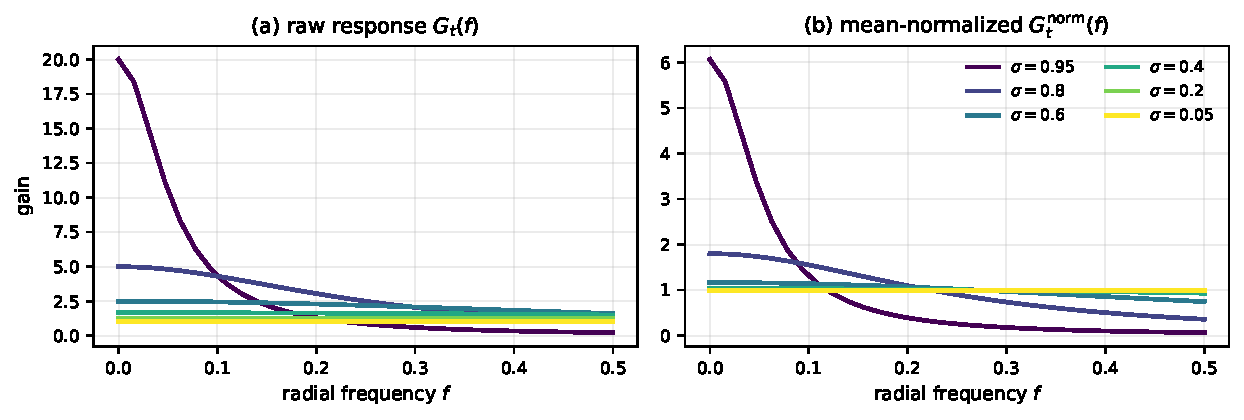
\includegraphics[width=0.95\linewidth]{figA_filters.pdf}
  \caption{Wiener filter responses along the flow schedule
  ($a_t = 1-\sigma$, $b_t = \sigma$, $S_x(f) = 1/|f|^p$, $p{=}2$ as used
  for FLUX; the video models use $p{=}3$ with the same qualitative
  shape). The formula is identical to SeaCache's; only the plotted
  schedule instance differs (flow, as used by our gate, vs.\ their
  DPM illustration). (a)~Raw response $G_t(f)$: low-pass early (large
  $\sigma$), widening as $\sigma \to 0$. (b)~Mean-normalized
  $G_t^{\mathrm{norm}}(f)$: comparable energy across timesteps, so
  accumulated distances are not dominated by gain drift. Computed from
  the closed form of~\eqref{eq:wiener}.}
  \label{fig:app-filters}
\end{figure}

%----------------------------------------------------------------
\section{Predictor hierarchy}
\label{app:hierarchy}

This section proves the three skip-length claims of
Secs.~\ref{sec:hierarchy}--\ref{sec:cheb}: copy-reuse is at most linear
in the skip length, degree-$P$ Taylor remainder is of order $P{+}1$, and
the Chebyshev truncation error does not depend on the skip length.
Throughout, $t_k$ is the last evaluated step and $t_j$ is the skipped
step at which the residual is reconstructed. The analysis is
channel-wise, as in the main text. The order-$P$ Taylor and Chebyshev
truncation statements are those of \citet[Thms.~3.1 and~3.2]{spectrum},
restated here for the residual trajectory $r$ in place of the hidden
state; the copy-reuse bound and the node-spacing refinement of the
discrete Taylor predictor are elementary.

\paragraph{Copy-reuse: linear bound.}
\label{app:reuse}
Copy-reuse sets $\hat{r}(t_j) = r(t_k)$. Assume $r$ is $L$-Lipschitz on
the sampling interval. Directly from the definition of Lipschitz
continuity,
\begin{equation}
  |r(t_j) - r(t_k)| \le L\,|t_j - t_k|,
\end{equation}
which is~\eqref{eq:reuse}. The bound is tight: $r(t) = Lt$ attains
equality for every skip. Lipschitz continuity is also necessary in the
worst case, since for a non-Lipschitz residual the ratio
$|r(t_j) - r(t_k)|/|t_j - t_k|$ is unbounded as the skip shrinks.
Copy-reuse uses no derivative
information, so additional smoothness ($r \in C^P$ for $P \ge 1$) cannot
improve this worst-case rate.

\paragraph{Taylor extrapolation: order-$(P{+}1)$ remainder.}
\label{app:taylor}
Assume $r \in C^{P+1}$. The degree-$P$ Taylor expansion of $r$ about
$t_k$ reads
\begin{equation}
  r(t_j)
  = \sum_{p=0}^{P} \frac{r^{(p)}(t_k)}{p!}\,(t_j-t_k)^p
  + R_P(t_j),
\end{equation}
with Lagrange remainder
\begin{equation}
  R_P(t_j)
  = \frac{r^{(P+1)}(\xi)}{(P{+}1)!}\,(t_j-t_k)^{P+1}
\end{equation}
for some $\xi$ between $t_k$ and $t_j$. Hence
$|R_P(t_j)| \le \frac{\|r^{(P+1)}\|_\infty}{(P{+}1)!}\,|t_j-t_k|^{P+1}$,
a $(P{+}1)$-order dependence on the skip length. This is the ideal
predictor: it uses the exact derivatives at $t_k$, which a
training-free cache never computes. In the discrete implementation the
derivatives $r^{(p)}(t_k)$ are replaced by backward differences
$\Delta^p r/(\Delta t)^p$ formed from $P{+}1$ neighboring evaluated
residuals $s_0 {=} t_k, s_1, \dots, s_P$, so the predictor is the
degree-$P$ interpolant $p_P$ through those nodes, with remainder
\begin{equation}
  r(t_j) - p_P(t_j)
  = \frac{r^{(P+1)}(\xi)}{(P{+}1)!}\prod_{q=0}^{P}(t_j - s_q)
  \label{eq:app-interp}
\end{equation}
for some $\xi$ in the convex hull of $\{t_j, s_0, \dots, s_P\}$. Only
the $q{=}0$ factor shrinks with the skip length
$\ell = |t_j - t_k|$; the remaining factors are fixed by the positions
of the earlier evaluated nodes. The $(P{+}1)$-order rate therefore
requires the node-spacing condition
$\max_q |t_j - s_q| \le C_{\mathrm{node}}\,\ell$, under which
$|r(t_j) - p_P(t_j)| \le C_{\mathrm{node}}^{P+1}
\|r^{(P+1)}\|_\infty \ell^{P+1}/(P{+}1)!$. The dynamic schedule does
not guarantee a uniform $C_{\mathrm{node}}$: with the earlier nodes
held fixed and $\ell \to 0$ the error is $O(\ell)$, not
$O(\ell^{P+1})$. The failure is sharp, not a loose estimate. Take
$P = 1$, $r(t) = t^2$, nodes $s_0 = t_k = 0$ and $s_1 = -H$ with
$H > 0$, and forecast point $t_j = \ell > 0$. The linear interpolant
through $(0,0)$ and $(-H,H^2)$ is $p_1(t) = -Ht$, so
$|r(\ell) - p_1(\ell)| = \ell(\ell + H)$ and
\begin{equation}
  \frac{|r(\ell) - p_1(\ell)|}{\ell^2} = 1 + \frac{H}{\ell},
  \label{eq:app-counterexample}
\end{equation}
which is unbounded as $H/\ell \to \infty$: no uniform constant over
arbitrary node configurations yields a bound of the form
$|r(t_j) - p_P(t_j)| \le C\,\ell^{P+1}$. Even uniform backward spacing
does not recover the ideal rate: for $t_j = t_k + \ell$ and
$s_q = t_k - qh$ with $h > 0$,
\begin{equation}
  \prod_{q=0}^{P}|t_j - s_q| = \prod_{q=0}^{P}(\ell + qh),
  \label{eq:app-uniform-product}
\end{equation}
a degree-$(P{+}1)$ polynomial in $\ell$ that coincides with
$\ell^{P+1}$ only in the limit $h/\ell \to 0$. In addition, the difference
operator amplifies observation noise by binomial coefficients of order
$2^P$. A higher $P$ therefore tightens the bound only for short skips
and becomes unstable as $|t_j-t_k|$ grows. The predictor also uses only
the $P{+}1$ most recent evaluations, discarding earlier trajectory
information.

\paragraph{Chebyshev truncation: skip-length-independent bound.}
\label{app:cheb}
Map the solver index to $\tau \in [-1,1]$ by an affine change of
variable, and write $r$ for the residual as a function of $\tau$. Let
$E_\rho$, $\rho > 1$, be the Bernstein ellipse with foci $\pm 1$ and
semi-axis sum $\rho$, and assume $r$ extends analytically to $E_\rho$
with $|r| \le B$ there. The Chebyshev coefficients then admit the
contour representation
$c_m = \frac{1}{\pi i}\oint_{E_\rho} r(z)\,T_m(z)^{-1}\,dz/z$ up to the
standard $m=0$ factor. On $E_\rho$ one has
$|T_m| \ge (\rho^m - \rho^{-m})/2$, which yields $|c_m| \le 2B\rho^{-m}$
for $m \ge 1$ and $|c_0| \le B$. Since $|T_m(\tau)| \le 1$ on $[-1,1]$,
truncating at degree $M$ leaves
\begin{equation}
  \|r - p_M^\star\|_\infty \le \sum_{m=M+1}^{\infty} 2B\rho^{-m}
  = \frac{2B}{\rho - 1}\,\rho^{-M},
\end{equation}
which is~\eqref{eq:cheb}. The right-hand side depends on $M$, $\rho$,
and $B$, but not on the evaluation point $\tau_j$. Consequently the
approximation-theoretic term is independent of the skip length
$|t_j-t_k|$. (The finite-sample ridge deviation from $p_M^\star$ is
controlled separately by Lemma~\ref{lem:ridge}.)

\paragraph{Node spacing versus design conditioning.}
The relative node-spacing condition above and the design-conditioning
quantity $\sigma_{\min}(\mathbf{\Phi})$ of Lemma~\ref{lem:ridge} are
distinct properties of the realized schedule: the former governs the
local interpolation remainder, the latter the stability of the fitted
Chebyshev coefficients, and neither implies the other. For one
direction, let the forecast distance $\ell > 0$ stay fixed while the
earlier nodes coalesce onto $t_k$; then
$\max_q|t_j - s_q|/\ell \to 1$, so the spacing condition holds with
$C_{\mathrm{node}} \to 1$, yet under the fixed affine normalization
the rows of $\mathbf{\Phi}$ become nearly identical and
$\sigma_{\min}(\mathbf{\Phi}) \to 0$ for any nonconstant basis.
Conversely, a fixed well-spread $K$-point design keeps
$\sigma_{\min}$ bounded away from zero while a forecast with
$\ell \to 0^+$ against a fixed distant node drives
$\max_q|t_j - s_q|/\ell \to \infty$. The ridge analysis of
Lemma~\ref{lem:ridge} is therefore not redundant alongside the
interpolation analysis: each controls a separate failure mode.

%----------------------------------------------------------------
\section{Proof of Lemma~\ref{lem:ridge} (ridge stability)}
\label{app:ridge}

The statement is Theorem~3.3 of \citet{spectrum}. We reproduce the
argument for the residual trajectory $r$ in place of the hidden state,
carrying the constants explicitly.

Fix one residual channel and drop the channel index, and take
$\lambda > 0$. Write the $K$
observations as $\mathbf{y} = \mathbf{\Phi}\mathbf{c}^\star + \mathbf{e}$,
where $\mathbf{c}^\star$ are the exact Chebyshev coefficients of
$p_M^\star$ and, by~\eqref{eq:cheb}, each entry of $\mathbf{e}$ satisfies
$|e_k| \le \varepsilon_M$, so $\|\mathbf{e}\|_2 \le \sqrt{K}\,\varepsilon_M$.
The ridge estimate is
$\hat{\mathbf{c}} = (\mathbf{\Phi}^\top\mathbf{\Phi} + \lambda I)^{-1}
\mathbf{\Phi}^\top \mathbf{y}$, hence
\begin{equation}
  \hat{\mathbf{c}} - \mathbf{c}^\star
  = (\mathbf{\Phi}^\top\mathbf{\Phi} + \lambda I)^{-1}\mathbf{\Phi}^\top \mathbf{e}
  - \lambda(\mathbf{\Phi}^\top\mathbf{\Phi} + \lambda I)^{-1}\mathbf{c}^\star.
  \label{eq:app-split}
\end{equation}
The forecast error at $\tau_j$ is the inner product of
$\hat{\mathbf{c}} - \mathbf{c}^\star$ with the basis row vector
$\boldsymbol{\phi}(\tau_j) = [T_0(\tau_j), \dots, T_M(\tau_j)]$, and
$|T_m| \le 1$ on $[-1,1]$ gives
$\|\boldsymbol{\phi}(\tau_j)\|_2 \le \sqrt{M{+}1\strut}$. Let
$\sigma_1 \ge \dots \ge \sigma_{M+1} = \sigma_{\min}$ be the singular
values of $\mathbf{\Phi} \in \mathbb{R}^{K \times (M+1)}$, with
$\sigma_{\min} = 0$ whenever $K < M{+}1$. We bound the two terms
of~\eqref{eq:app-split} in turn.

\paragraph{Variance term.} In the singular-value decomposition of
$\mathbf{\Phi}$,
\begin{equation}
  \|(\mathbf{\Phi}^\top\mathbf{\Phi} + \lambda I)^{-1}\mathbf{\Phi}^\top\|_2
  = \max_i \frac{\sigma_i}{\sigma_i^2 + \lambda}
  \le \frac{\sigma_1}{\sigma_{\min}^2 + \lambda},
\end{equation}
and every entry of $\mathbf{\Phi}$ is bounded by one, so
$\sigma_1 \le \|\mathbf{\Phi}\|_F \le \sqrt{(M{+}1)K}$. Combining this
with $\|\boldsymbol{\phi}(\tau_j)\|_2 \le \sqrt{M{+}1\strut}$ and
$\|\mathbf{e}\|_2 \le \sqrt{K}\,\varepsilon_M$,
\begin{equation}
  \bigl|\boldsymbol{\phi}(\tau_j)
  (\mathbf{\Phi}^\top\mathbf{\Phi} + \lambda I)^{-1}\mathbf{\Phi}^\top \mathbf{e}\bigr|
  \le \sqrt{M{+}1\strut}\cdot\frac{\sqrt{(M{+}1)K}}{\sigma_{\min}^2 + \lambda}
      \cdot\sqrt{K}\,\varepsilon_M
  = \frac{(M{+}1)K}{\sigma_{\min}^2 + \lambda}\,\varepsilon_M.
\end{equation}

\paragraph{Bias term.} The Chebyshev coefficients of a function
analytic on $E_\rho$ and bounded by $B$ there satisfy
$|c^\star_m| \le 2B\rho^{-m}$ (App.~\ref{app:cheb}), so
\begin{equation}
  \|\mathbf{c}^\star\|_2
  \le 2B\Bigl(\sum_{m \ge 0}\rho^{-2m}\Bigr)^{1/2}
  = \frac{2B}{\sqrt{1-\rho^{-2}}},
\end{equation}
a bound independent of $M$. Since the eigenvalues of
$(\mathbf{\Phi}^\top\mathbf{\Phi} + \lambda I)^{-1}$ are
$1/(\sigma_i^2 + \lambda)$, its spectral norm is
$1/(\sigma_{\min}^2 + \lambda)$, and therefore
\begin{equation}
  \bigl|\boldsymbol{\phi}(\tau_j)\,
  \lambda(\mathbf{\Phi}^\top\mathbf{\Phi} + \lambda I)^{-1}\mathbf{c}^\star\bigr|
  \le \frac{\lambda\sqrt{M{+}1\strut}}{\sigma_{\min}^2 + \lambda}
      \cdot\frac{2B}{\sqrt{1-\rho^{-2}}}.
\end{equation}

\paragraph{Combination.} Adding the two bounds gives
Lemma~\ref{lem:ridge}. Adding $\varepsilon_M$ once more,
by~\eqref{eq:cheb} and the triangle inequality, bounds the total error
$|r(\tau_j) - \hat{r}(\tau_j)|$ and recovers Theorem~3.3
of \citet{spectrum}. The two terms expose the trade-off: further
observations raise $\sigma_{\min}$ and keep the variance factor
bounded, while $\lambda$ guards the rank-deficient regime $K < M{+}1$
at the price of bias.

%----------------------------------------------------------------
\section{Residual-space error identity and conditioning}
\label{app:residual}

On a skipped step the block input $\mathbf{h}_{\mathrm{in}}$ is known
exactly from the current sampling state and the preceding computation,
so with $\mathbf{h}_{\mathrm{out}} = \mathbf{h}_{\mathrm{in}} + \mathbf{r}$,
\begin{equation}
  \hat{\mathbf{h}}_{\mathrm{out}} - \mathbf{h}_{\mathrm{out}}
  = \hat{\mathbf{r}} - \mathbf{r},
\end{equation}
i.e.\ state and residual forecasts share the same error for a fixed fit.
The fits differ in their regression target. Stacking the observed
input, output, and residual rows gives matrices satisfying the exact
identity $\mathbf{H}_{\mathrm{out}} = \mathbf{H}_{\mathrm{in}} +
\mathbf{R}$, where $\mathbf{H}_{\mathrm{in}}$ varies with the sampling
step and is not rank one, so no low-rank decomposition is assumed.
Each hidden-state observation carries the large input component, which
the sampler already knows exactly; fitting the full state therefore
inflates the regression target without adding anything that needs
predicting. The ridge map is linear in its target, so scaling the
target scales the fitted coefficients and the absolute shrinkage bias
while the shrinkage factor $\lambda/(\sigma_{\min}^2 + \lambda)$ is
unchanged (App.~\ref{app:ridge}): the ridge constants scale with the
target norm through $B$, which bounds the analytic continuation of the
fitted trajectory. Forecasting $\mathbf{R}$ directly keeps the target
small-normed and tightens every constant in proportion, a
target-scale advantage rather than a design-conditioning one --- all
fits share the same design matrix $\mathbf{\Phi}$ and hence identical
conditioning. The skipped-step update is $\mathbf{h} \gets
\mathbf{h} + \hat{\mathbf{r}}$.

%----------------------------------------------------------------
\section{Blend optimum and warm-up threshold}
\label{app:blend}

\paragraph{Blend weight.} With uncorrelated Taylor error (squared bias
$b_T^2$) and Chebyshev error (variance $\sigma_C^2$), the blended risk is
$R(w) = (1-w)^2 b_T^2 + w^2\sigma_C^2$. Setting $R'(w) = 0$ gives
$w^\star = b_T^2/(b_T^2 + \sigma_C^2)$. Early in sampling both the drift
and the fit variance are large; late in sampling both shrink as the
trajectory settles and $K$ grows (Appendix~\ref{app:ridge}).
Measured trajectories keep the two terms within a factor of two of each
other, which places $w^\star$ near $1/2$ throughout and motivates the
fixed $w = 0.5$.

\paragraph{Warm-up.} With $n$ observations and $M{+}1$ bases, $n < M{+}1$
leaves~\eqref{eq:ridge} rank-deficient: $\sigma_{\min}(\mathbf{\Phi}) =
0$, the observations cannot identify all coefficient directions, and the
fit is dominated by the prior (the bias term of
Appendix~\ref{app:ridge} governs). The first-order discrete Taylor step is
exact on the last two observations by construction and therefore
strictly dominates in this regime. Blending from $n \ge 4$ onward (the
$M = 4$ fit being determined in practice) is thus the degrees-of-freedom
crossover rather than a tuned choice.

%----------------------------------------------------------------
\section{Refresh-ratio analysis}
\label{app:refresh}
Refresh histograms concentrate compute early along the trajectory, in
accordance with the spectral prior of~\eqref{eq:wiener}: evaluations are
dense while $G_t$ is narrow (content forming) and sparse as the passband
widens. PSNR-versus-refresh curves for ReSPect follow the full-compute
reference monotonically at both $\delta$ settings, with the gap to
copy-reuse widening at lower refresh ratios, precisely where the reuse
bound~\eqref{eq:reuse} loosens and the uniform bound~\eqref{eq:cheb}
remains tight, as anticipated in Sec.~\ref{sec:t2i}.

\begin{figure}[h]
  \centering
  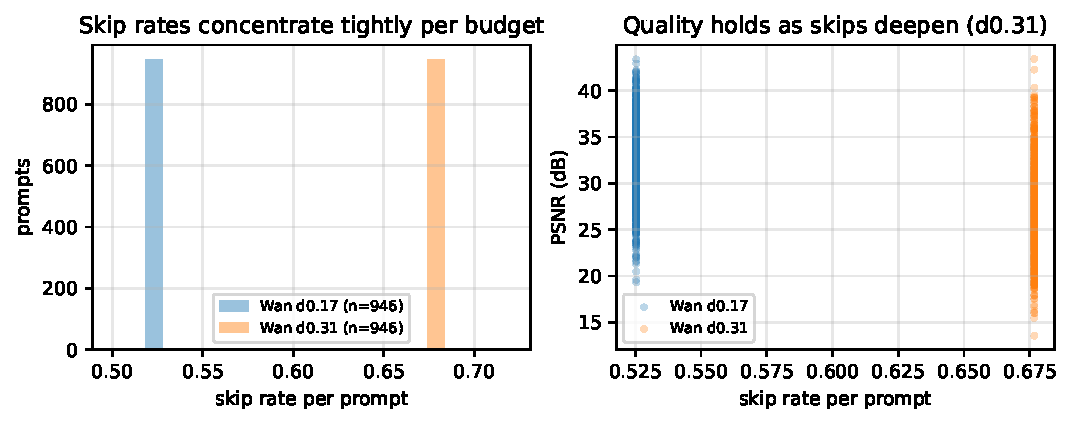
\includegraphics[width=0.95\linewidth]{figA_skip.pdf}
  \caption{Compute concentrates early; quality tracks full compute.
  Left: per-prompt skip-rate histograms (Wan). Right: per-prompt PSNR
  vs skip rate over full VBench-946.}
  \label{fig:app-refresh}
\end{figure}

\begin{figure}[h]
  \centering
  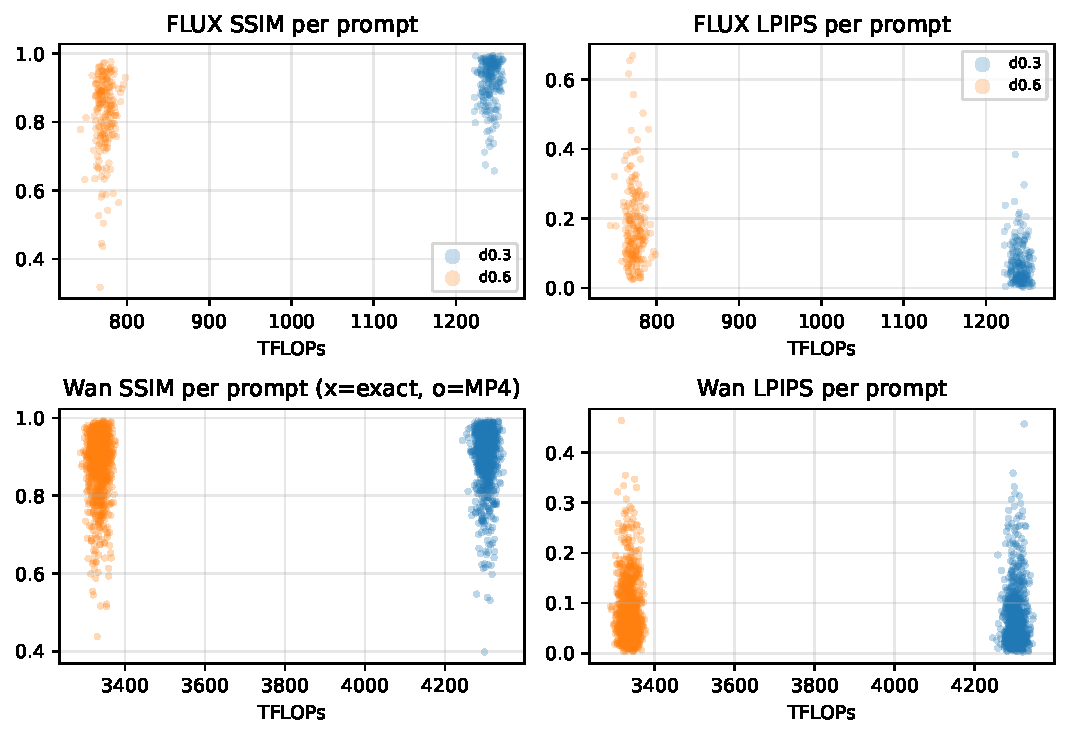
\includegraphics[width=0.95\linewidth]{figA_ssim_lpips.pdf}
  \caption{Per-prompt SSIM/LPIPS clouds at each config's TFLOPs.
  Top: FLUX DrawBench-200. Bottom: Wan VBench-946 .}
  \label{fig:app-clouds}
\end{figure}

%----------------------------------------------------------------
\section{Implementation details}
\label{app:impl}

\paragraph{Forecaster.} $M{=}4$ Chebyshev bases, window $K{=}100$,
$\lambda{=}0.1$, blend $w{=}0.5$, first-order discrete Taylor,
Taylor-only warm-up until $n \ge 4$ observations. Time is mapped to
$\tau \in [-1,1]$ over the fixed range $[0, 50]$ (buffer min/max is
\emph{not} used). One forecaster per sample; coefficient state is a single
$(M{+}1)\times F$ matrix plus $K$ cached residuals.

\paragraph{Complexity.} Fitting is $\mathcal{O}(K(M{+}1)F)$ with
$M \ll K \ll F$ (the $(M{+}1)^3$ Cholesky term is negligible);
prediction is $\mathcal{O}((M{+}1)F)$; memory is
$\mathcal{O}((M{+}1)F + KF)$. Measured overhead is ${\sim}0.09$\,s/image
on FLUX. First and last steps always compute; CFG call streams are
demuxed by timestep equality.

\paragraph{Hardware and seeds.} FLUX.1-dev, DrawBench (200 prompts),
$1024{\times}1024$, 50 steps, guidance 3.5, bf16, seeds $0{+}i$.
Video: VBench prompts, 480p, 65 frames, 50 steps. All latencies are
wall-clock on a single NVIDIA B200; all quality claims are at matched NFE.

%----------------------------------------------------------------
\paragraph{Cost of the forecaster.} A latency column combines the
effects of schedule and reconstructor, since two methods at the same budget
may skip at different steps. Running both reconstructors in one harness
at the same $\delta$, which fixes the schedule and varies only what is
written on a skipped step, yields identical realized NFE: the gate reads
the modulated block input, so replacing copy-reuse with a forecast does
not alter where it fires. The forecast adds $1.7$--$4.3\%$ wall-clock
over copy-reuse (Tab.~\ref{tab:overhead}).

\begin{table}[h]
  \centering
  \caption{Cost of the reconstructor at fixed schedule. Both columns of each
  row use the same gate and the same $\delta$ in the same harness on one
  B200; only the skipped-step reconstruction differs. NFE is identical
  within every pair.}
  \label{tab:overhead}
  \vspace{0.1cm}
  {\small\setlength{\tabcolsep}{5pt}
  \begin{tabular}{llcccc}
    \toprule
    Model & $\delta$ & NFE & Copy-reuse (s) & Forecast (s) & $\Delta$ \\
    \midrule
    FLUX.1-dev   & 0.3  & 21 & 2.38  & 2.47  & $+3.8\%$ \\
    FLUX.1-dev   & 0.6  & 13 & 1.55  & 1.61  & $+3.9\%$ \\
    Wan2.1-1.3B  & 0.17 & 46 & 14.31 & 14.80 & $+3.4\%$ \\
    Wan2.1-1.3B  & 0.31 & 32 & 10.49 & 10.94 & $+4.3\%$ \\
    HunyuanVideo & 0.27 & 24 & 39.20 & 39.86 & $+1.7\%$ \\
    HunyuanVideo & 0.48 & 16 & 27.38 & 27.90 & $+1.9\%$ \\
    \bottomrule
  \end{tabular}}
\end{table}

\paragraph{ReSPect vs.\ SeaCache at matched schedules.}
We further compare ReSPect against SeaCache~\citep{seacache} copy-reuse
under matched schedules, tuning $\delta$ to equalize NFE. Both arms run
in our own harness: the gate is unchanged, so the two methods realize
(near-)identical NFE and only the skipped-step reconstruction differs.
Tab.~\ref{tab:abl-sea} reports full-reference quality against the
uncached outputs. The forecast wins on PSNR, SSIM, and LPIPS at every
setting with a matched pair: $+0.79$\,dB on FLUX $\delta{=}0.37$
($n{=}200$), $+0.49$\,dB on FLUX $\delta{=}0.6$ ($n{=}20$), and
$+0.93$\,dB on Wan $\delta{=}0.31$ ($n{=}20$), with LPIPS down $18\%$
where measured. We attribute this to the residual forecast tracking
the trajectory between evaluations, whereas copy-reuse holds the last
observed residual fixed.

\begin{table}[h]
  \centering
  \caption{ReSPect vs.\ SeaCache copy-reuse at matched schedules: same
  $\delta$, same prompts, (near-)identical NFE; only the skipped-step
  reconstruction differs. LPIPS was not measured on the 20-prompt
  subsets (---). The FLUX $\delta{=}0.37$ pair is full DrawBench-200;
  the $\delta{=}0.6$ and Wan pairs are fixed 20-prompt subsets.}
  \label{tab:abl-sea}
  \vspace{0.1cm}
  {\scriptsize\setlength{\tabcolsep}{4pt}
  \begin{tabular}{llcccc}
    \toprule
    Setting & Method & NFE & PSNR$\uparrow$ & SSIM$\uparrow$  \\
    \midrule
    FLUX $\delta{=}0.37$ & SeaCache & 18.1 & 25.45 & 0.880  \\
    ($n{=}200$) & \textbf{ReSPect} & \textbf{18.1} & \textbf{26.24} & \textbf{0.895}  \\
    \midrule
    FLUX $\delta{=}0.6$ & SeaCache & 13.0 & 23.08 & 0.848  \\
    ($n{=}20$) & \textbf{ReSPect} & \textbf{13.0} & \textbf{23.57} & \textbf{0.852} \\
    \midrule
    Wan $\delta{=}0.31$ & SeaCache & 32.4 & 28.80 & 0.904  \\
    ($n{=}20$) & \textbf{ReSPect} & \textbf{32.3} & \textbf{29.73} & \textbf{0.917} &  \\
    \bottomrule
  \end{tabular}}
\end{table}

\section{Reconstructor ablations against copy-reuse}
\label{app:abl-reuse}

All arms share one base run, so every $\Delta$dB value below is paired
against the same copy-reuse baseline (Fig.~\ref{fig:ablation}), run at
the aggressive budgets (FLUX $\delta{=}0.6$, Wan $\delta{=}0.31$) on
fixed 20-prompt subsets.

\paragraph{Blend weight $w$.}
Pure Taylor ($w{=}0$) is strong wherever neighboring evaluations carry
the signal: $+2.30$\,dB on Wan and $+0.50$\,dB on FLUX. Pure Chebyshev
($w{=}1$) fails precisely where the fit is least determined:
$-1.68$\,dB on Wan, with its long skip runs, and $+0.09$\,dB
($\approx$ copy-reuse) on FLUX. The fixed $w{=}0.5$ remains at or above
copy-reuse on either model ($+0.49$/$+0.93$\,dB); it is a robust
compromise, and the setting used in the main tables, rather than a
per-subset optimum.

\paragraph{Warm-up threshold.}
Blending before the fit is determined ($n < M{+}1$) lets the penalty
dominate the data. A warm-up of 8 attains the largest FLUX gain
($+0.68$\,dB) but lies within noise of the default blend; longer
Taylor-only spans (12--24) never accumulate enough observations to
blend at this budget and coincide with pure Taylor ($+0.50$\,dB).
Extending the warm-up is therefore without penalty, and the polynomial term
engages only once the fit is determined.

\paragraph{Window $K$.}
$K{=}32$ matches $K{=}100$ to three decimals ($+0.491$ vs.\
$+0.491$\,dB): per-prompt buffers rarely exceed ${\sim}40$
observations, so the $\sigma_{\min}$ gains of Lemma~\ref{lem:ridge}
have saturated early and $K{=}100$ is a conservative default rather than a
tuned choice.

\begin{figure}[h]
  \centering
  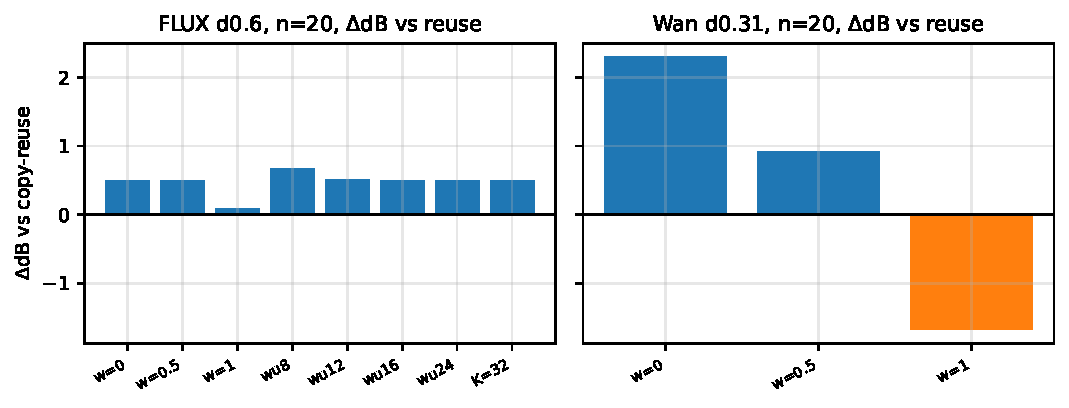
\includegraphics[width=0.9\linewidth]{figs/fig_ablation.pdf}
  \caption{Ablations ($\Delta$dB against copy-reuse, paired on one
  shared base run per panel). Left: FLUX $\delta{=}0.6$, $n{=}20$.
  Right: Wan $\delta{=}0.31$, $n{=}20$. Pure Taylor dominates on Wan
  while the blend remains at or above copy-reuse; pure Chebyshev fails on
  long skip runs; warm-ups of 12 and above never engage the blend; the
  window $K$ has saturated.}
  \label{fig:ablation}
\end{figure}

\section{Additional qualitative results}
\label{app:qual}

\begin{figure}[h]
  \centering
  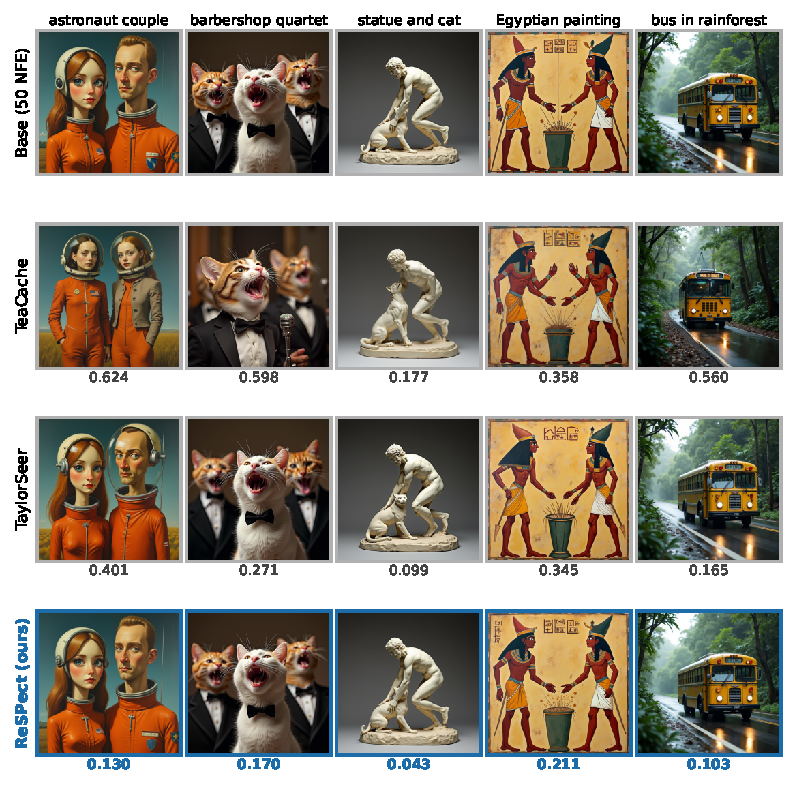
\includegraphics[width=\linewidth]{figs/fig_qual_flux.pdf}
  \caption{FLUX.1-dev at the aggressive budget, all methods run in our
  harness. ReSPect at $\delta{=}0.6$; TaylorSeer ($\mathcal{S}{=}5$) and
  TeaCache ($\delta{=}0.6$) use equal or more compute. LPIPS against the
  base image is printed under each panel. Over 20 DrawBench prompts
  ReSPect attains the lowest LPIPS on 19 (mean $0.183$ vs.\ $0.256$ and
  $0.407$).}
  \label{fig:qual}
\end{figure}

\begin{figure}[h]
  \centering
  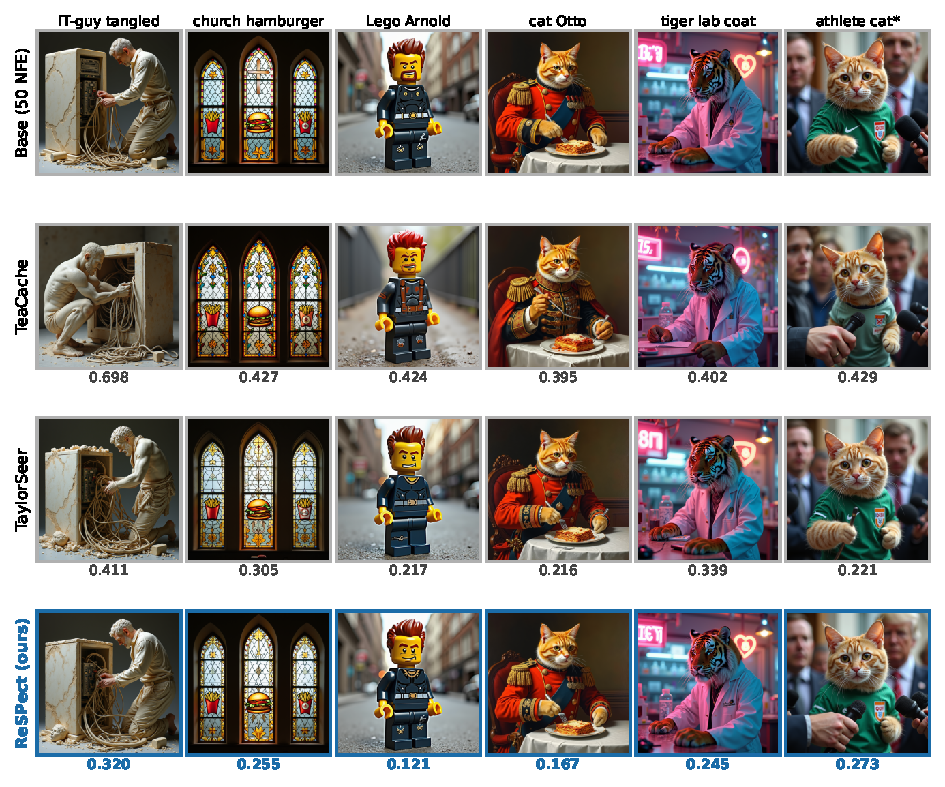
\includegraphics[width=\linewidth]{figs/fig_qual_flux_b.pdf}
  \caption{Six further DrawBench prompts at the same aggressive budget
  and harness as Fig.~\ref{fig:qual} (ReSPect $\delta{=}0.6$;
  TaylorSeer $\mathcal{S}{=}5$; TeaCache $\delta{=}0.6$). ReSPect is
  closest to the base on five of six; ``athlete cat*'' is the single
  prompt of the twenty where TaylorSeer attains the lower LPIPS
  ($0.221$ vs.\ $0.273$), shown here for completeness.}
  \label{fig:qual-b}
\end{figure}

All clips below are generated in our harness on one B200. ReSPect runs
at $\delta{=}0.31$ (Wan, 32 forward passes) and $\delta{=}0.48$
(Hunyuan, 16); TeaCache and TaylorSeer run at their published operating
points and use more compute . The two
sentence prompts are (retriever) ``A golden retriever running along a
sandy beach at sunset, waves rolling in behind it'' and (balloon) ``A
red hot air balloon drifting slowly over green rolling hills under a
clear blue sky''; both are also printed in the title of each strip
figure. Per-frame PSNR against the base frame is printed under each
panel. Averaged over all 65 frames, ReSPect leads on every clip:
Wan balloon $34.87$ vs.\ $31.29$ / $17.60$; Wan retriever $30.96$ vs.\
$27.07$ / $17.91$; Hunyuan balloon $37.41$ vs.\ $25.80$ / $21.52$;
Hunyuan retriever $26.04$ vs.\ $16.32$ / $15.24$
(TeaCache / TaylorSeer). The retriever prompt is a difficult motion
case in which all caches degrade while the ordering is preserved.
Tab.~\ref{tab:app-qual} gives the full per-prompt comparison with SSIM
and LPIPS (frame-averaged against the uncached same-seed reference).

\begin{table}[h]
  \centering
  \caption{Per-prompt qualitative-clip comparison: frame-averaged PSNR,
  SSIM, and LPIPS against the uncached same-seed reference over all 65
  frames. NFE is forward passes per clip (Wan base 100, Hunyuan base
  50). ReSPect uses the least compute and leads on every clip and
  metric.}
  \label{tab:app-qual}
  \vspace{0.1cm}
  {\scriptsize\setlength{\tabcolsep}{3pt}
  \begin{tabular}{llcccc}
    \toprule
    Clip & Method & PSNR$\uparrow$ & SSIM$\uparrow$ & LPIPS$\downarrow$ & NFE \\
    \midrule
    Wan retriever & TeaCache & 27.07 & 0.892 & 0.109 & 38 \\
    & TaylorSeer & 17.91 & 0.656 & 0.384 & 36 \\
    & \textbf{ReSPect} & \textbf{30.96} & \textbf{0.937} & \textbf{0.066} & \textbf{32} \\
    \midrule
    Wan balloon & TeaCache & 31.29 & 0.918 & 0.064 & 38 \\
    & TaylorSeer & 17.60 & 0.568 & 0.321 & 36 \\
    & \textbf{ReSPect} & \textbf{34.87} & \textbf{0.950} & \textbf{0.031} & \textbf{32} \\
    \midrule
    Hunyuan retriever & TeaCache & 16.32 & 0.669 & 0.322 & 18 \\
    & TaylorSeer & 15.24 & 0.643 & 0.379 & 18 \\
    & \textbf{ReSPect} & \textbf{26.04} & \textbf{0.878} & \textbf{0.089} & \textbf{16} \\
    \midrule
    Hunyuan balloon & TeaCache & 25.80 & 0.914 & 0.046 & 18 \\
    & TaylorSeer & 21.52 & 0.903 & 0.117 & 18 \\
    & \textbf{ReSPect} & \textbf{37.41} & \textbf{0.980} & \textbf{0.005} & \textbf{16} \\
    \bottomrule
  \end{tabular}}
\end{table}

\begin{figure}[h]
  \centering
  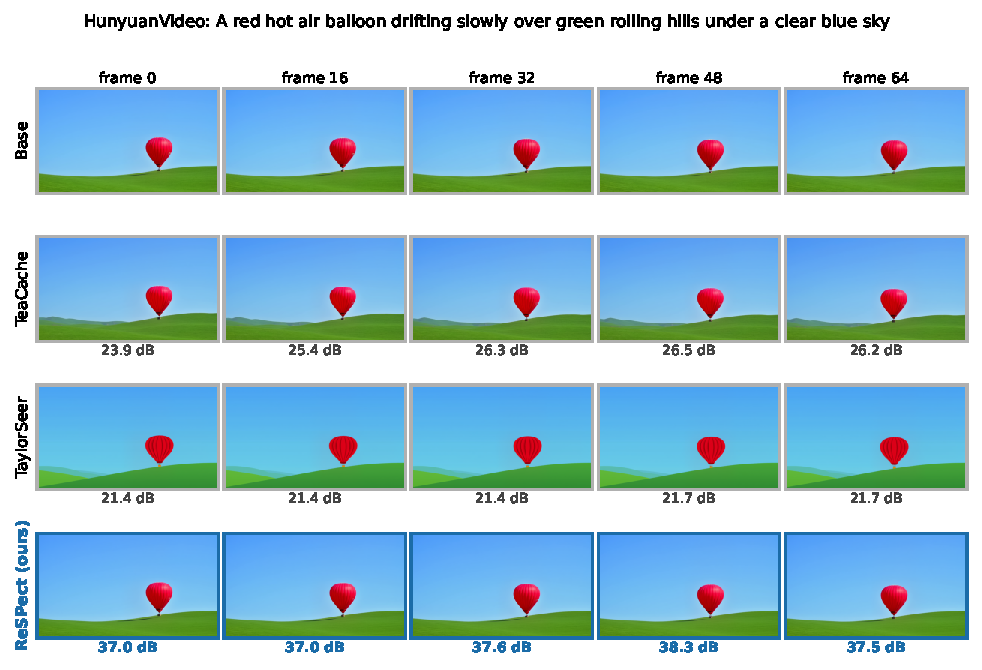
\includegraphics[width=\linewidth]{figs/fig_seq_hunyuan_p1.pdf}
  \caption{HunyuanVideo, balloon clip, $\delta{=}0.48$ (16 NFE).
  TaylorSeer renders a different scene entirely and retains it for the
  whole clip; averaged over all 65 frames, ReSPect scores $37.41$\,dB
  against $25.80$ (TeaCache) and $21.52$ (TaylorSeer).}
  \label{fig:app-qual-hun1}
\end{figure}

\begin{figure}[h]
  \centering
  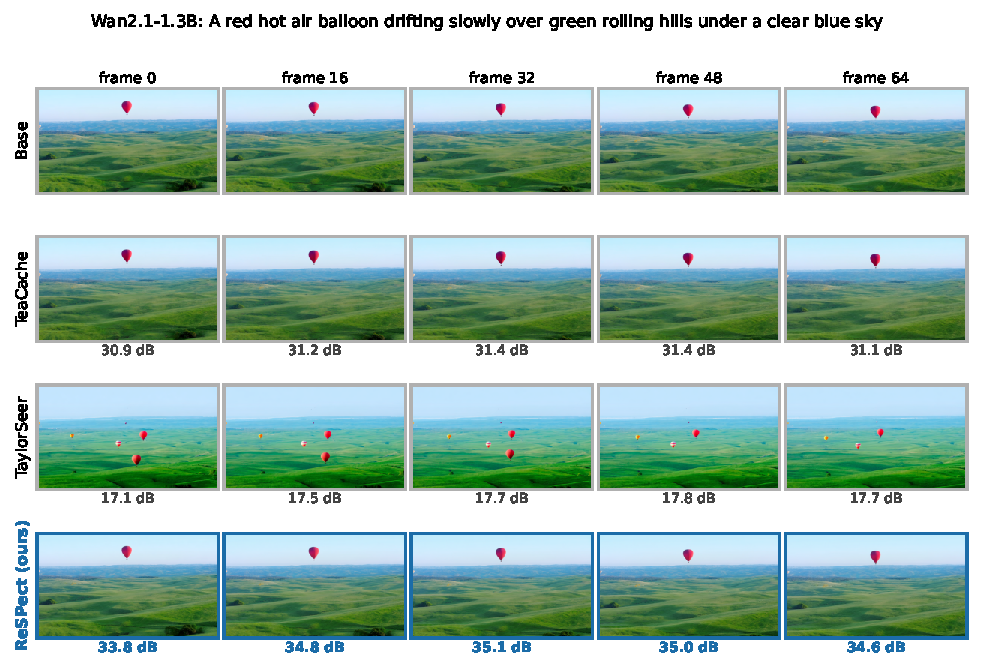
\includegraphics[width=\linewidth]{figs/fig_seq_wan_p1.pdf}
  \caption{Wan2.1, balloon clip, $\delta{=}0.31$ (32 NFE).
  TaylorSeer hallucinates three additional balloons
  and retains them for the whole clip.}
  \label{fig:app-qual}
\end{figure}

\begin{figure}[h]
  \centering
  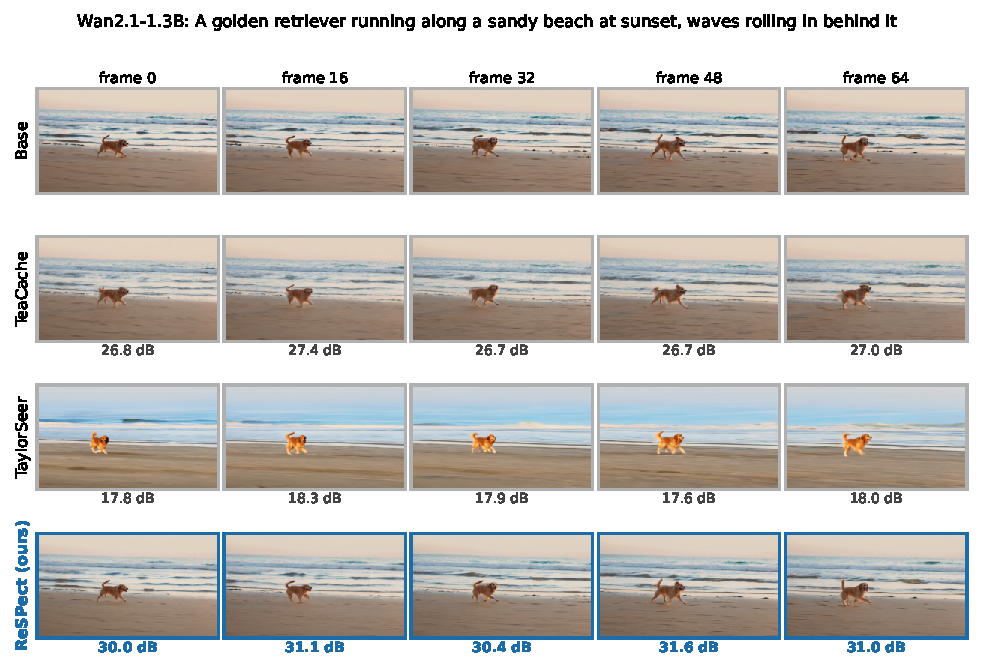
\includegraphics[width=\linewidth]{figs/fig_seq_wan_p0.pdf}
  \caption{Wan2.1, retriever clip, $\delta{=}0.31$ (32 NFE): a difficult
  motion prompt. All methods lie closer to the base here; the forecast
  still gains $+3.9$\,dB over the next baseline, whereas the
  interval-based and raw-distance schedules lose $4$--$13$\,dB.}
  \label{fig:app-qual-wan0}
\end{figure}

\begin{figure}[h]
  \centering
  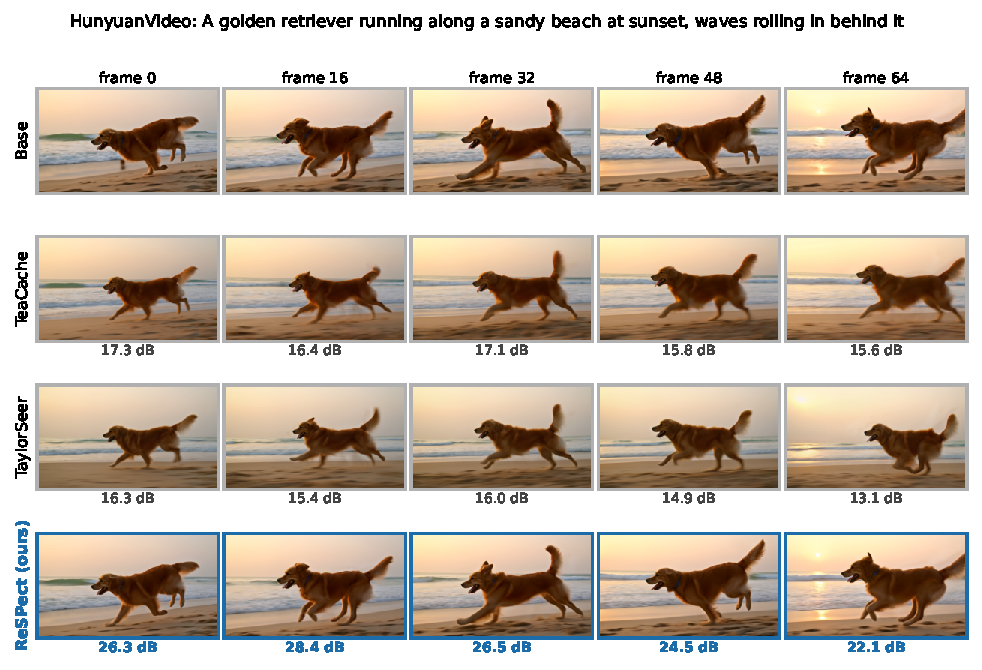
\includegraphics[width=\linewidth]{figs/fig_seq_hunyuan_p0.pdf}
  \caption{HunyuanVideo, retriever clip, $\delta{=}0.48$ (16 NFE).}
  \label{fig:app-qual-hun0}
\end{figure}



\end{document}
